\chapter{Results}
In this section, results from the computation using the implemented software are presented. There are two classical benchmarks for 3-dimensional MHD equations, namely the MHD Blast \cite{blast1}, \cite{blast2}, and the Orszag-Tang vortex \cite{vortex}. And then the main section of this work contains results from the flux tube eruption model on and above the Sun's surface.

\section{Benchmarks}
The benchmarks presented in this Section do not have an exact analytical solution, but the formation of waves and discontinuities is well studied, and benchmarking is usually performed on the basis of comparing the structure and presence of non-physical attributes.
\subsection{MHD Blast}
\subsubsection{MHD Blast - original version}
This benchmark has been used for decades - \cite{blast0}, \cite{blast1}, \cite{blast2} - in a variety of configurations and as a benchmark in software - e.g. \citep{athena}. The setup as described in \cite{blast0}, \cite{blast1} is defined (although in \cite{blast1} with interchanged $x-$ and $y-$ coordinates) by the initial conditions:
\begin{align}
\label{mhdBlastOld}
\gamma & =  5 / 3\\ \nonumber
p_0\lo\bfx, t\ro & =  100\ \ \text{for}\ \left|\bfx\right| < 0.1\\ \nonumber
p_0\lo\bfx, t\ro & =  1\ \ \text{for}\ \left|\bfx\right| \geq 0.1\\ \nonumber
\rho\lo\bfx, t = 0\ro & =  1,\\ \nonumber
p\lo\bfx, t = 0\ro & =  p_0\lo\bfx, t\ro,\\ \nonumber
\bfu_1\lo\bfx, t = 0\ro & =  0,\\ \nonumber
\bfu_2\lo\bfx, t = 0\ro & =  0,\\ \nonumber
\bfu_3\lo\bfx, t = 0\ro & =  0,\\ \nonumber
\bfB_1\lo\bfx, t = 0\ro & =  0,\\ \nonumber
\bfB_2\lo\bfx, t = 0\ro & =  100,\\ \nonumber
\bfB_3\lo\bfx, t = 0\ro & =  0.
\end{align}
Total energy is calculated using \Cref{magU}, \Cref{kinU}, \Cref{presU}.
The domain $\Omega$ is a square, with scaling quite arbitrarily used in the papers. In the case of \cite{blast1}, $\Omega = [0, 1] \times [0, 1]$, in this work it is $\Omega = [-0.25, 0.25] \times [-0.25, 0.25]$.

It is obvious from the initial setup, that the example is true to its name, and it is in fact a blast of the over-pressured area $\left|\bfx\right| < 0.1$, where pressure $p$ is 100$\times$ larger than elsewhere in the domain. This setup is completed with simple outflow boundary condition \Cref{bcoutdef}.
In the next figures, the solution as presented in \cite{blast1} is compared to the solution obtained with the approach described in this work. Note that the solution from \cite{blast1} needed to have the axes transformed $\lo x\rightleftharpoons y\ro$ with respect to the original paper. The figure \Cref{figure:blastOldRef} is taken from the article \cite{blast1} from the page 33. Unfortunately the paper does not specify the precise time at which the snapshots are taken.

\begin{figure}[H]
\centering
\hspace{-8mm}
\subfigure{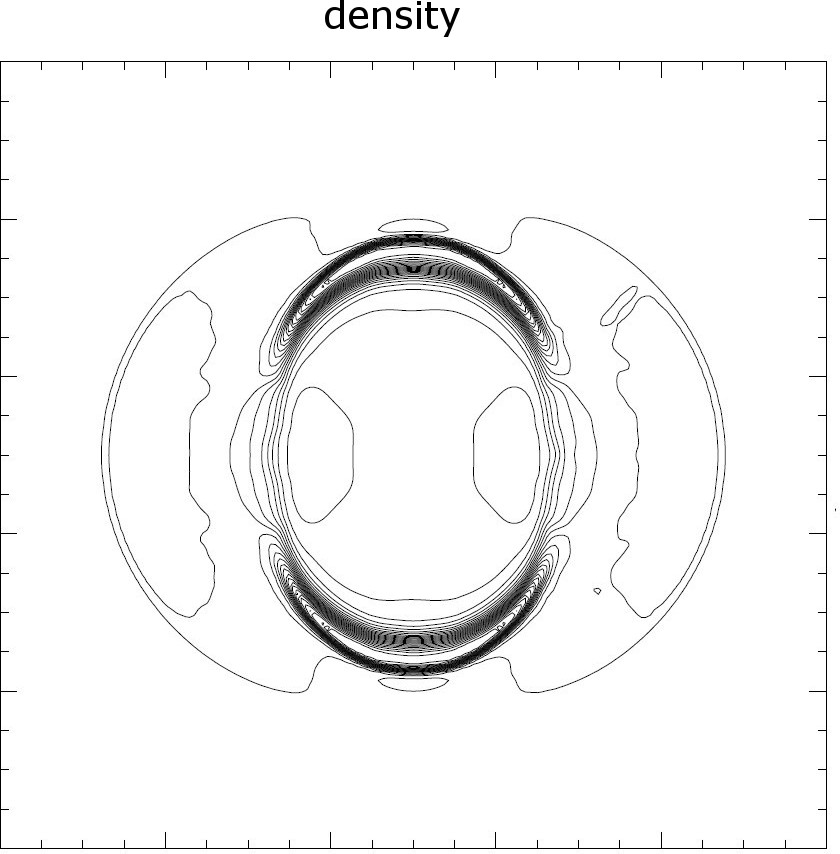
\includegraphics[width=0.4\textwidth]{img/mhd-blast/old/ref.jpg}}
\subfigure{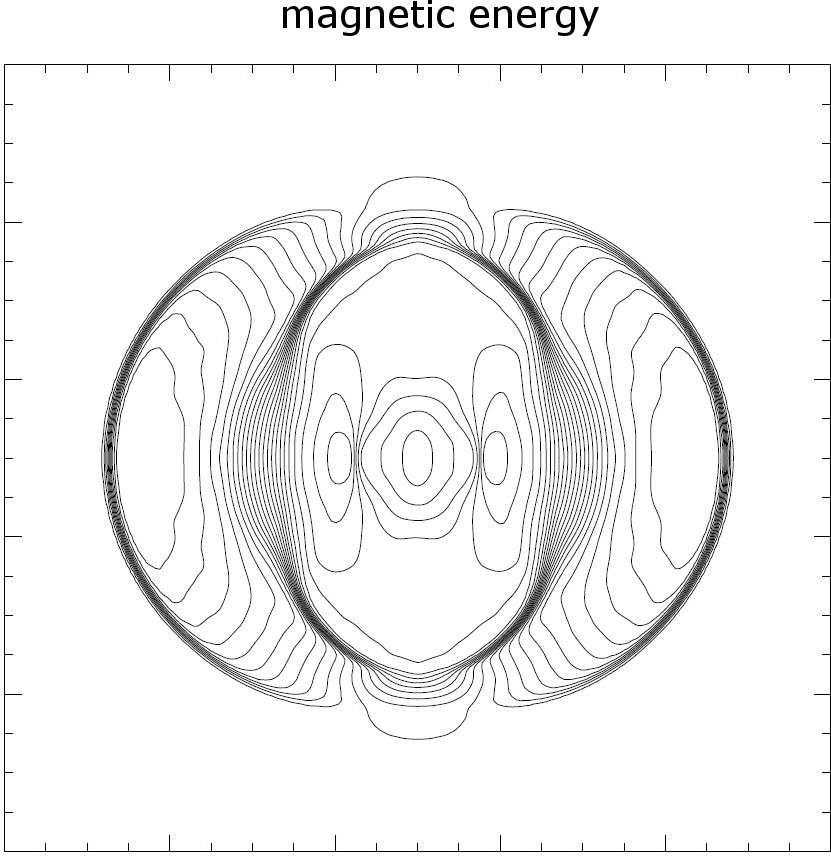
\includegraphics[width=0.395\textwidth]{img/mhd-blast/old/refmag.jpg}}
\caption{Results from \cite{blast1}, density(left), magnetic energy(right)}
\label{figure:blastOldRef}
\end{figure}

\vspace{-5mm}
\begin{figure}[H]
	\begin{center}
		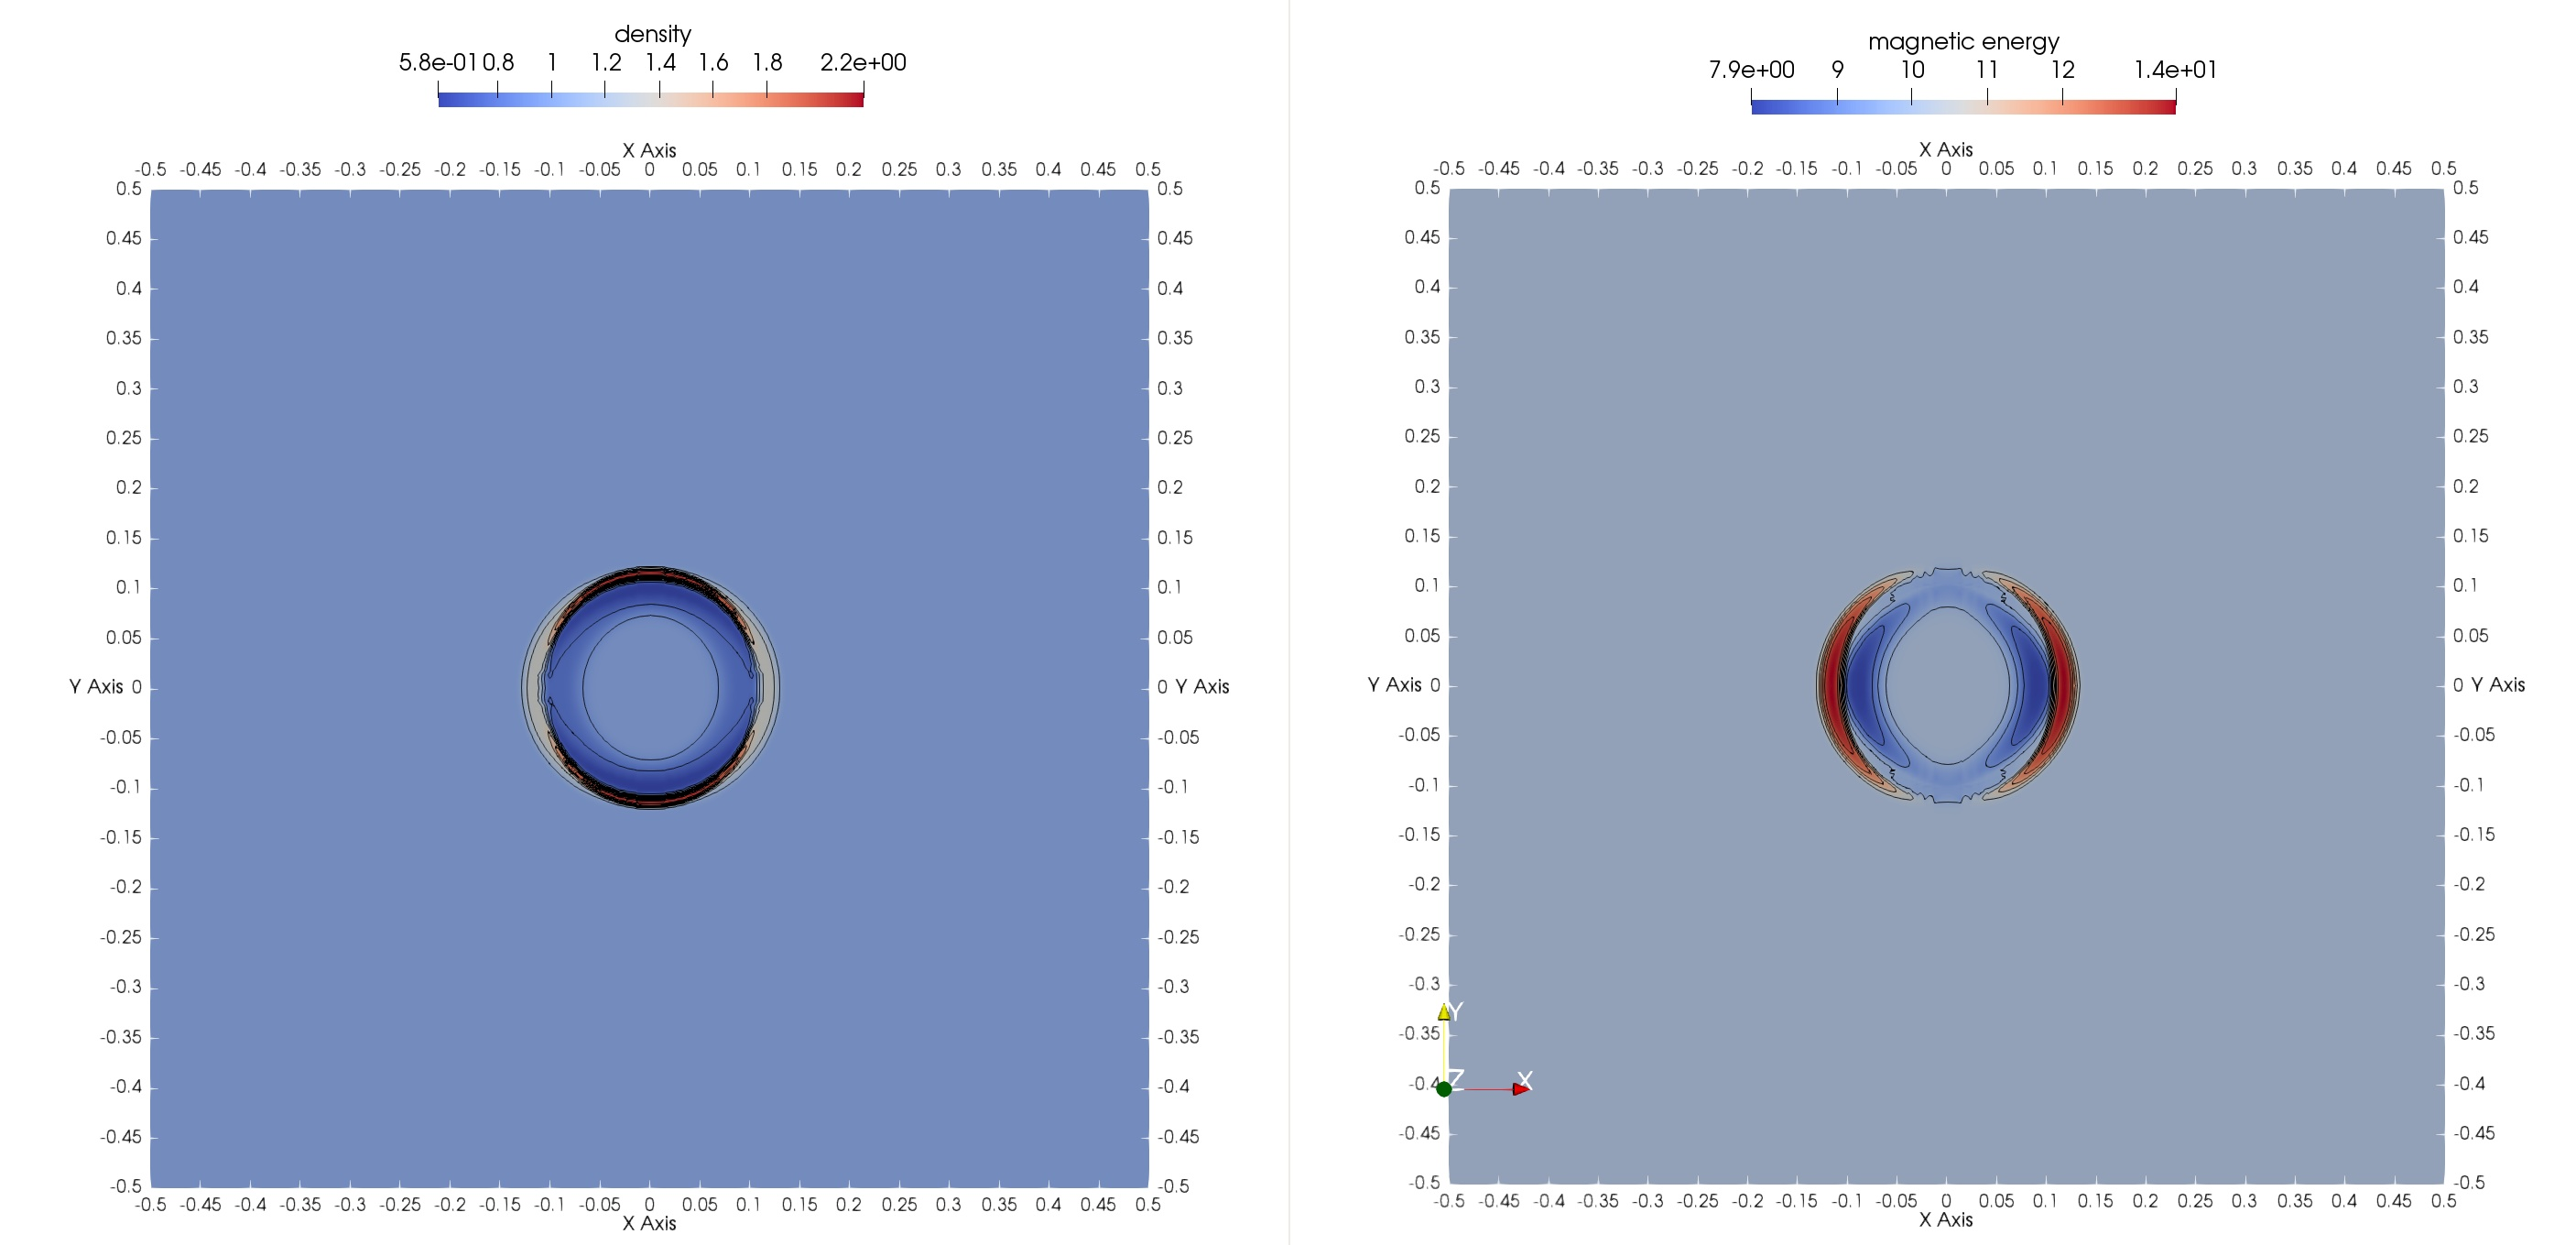
\includegraphics[width=0.87\textwidth]{img//mhd-blast/old/mynew1.jpg}
	\caption{Obtained results, $t = 1\times 10^{-3}$, density(left), magnetic energy(right)}
	\label{figure:blastOldMy1}
	\end{center}
\end{figure}
\vspace{-8mm}

\begin{figure}[H]
	\begin{center}
		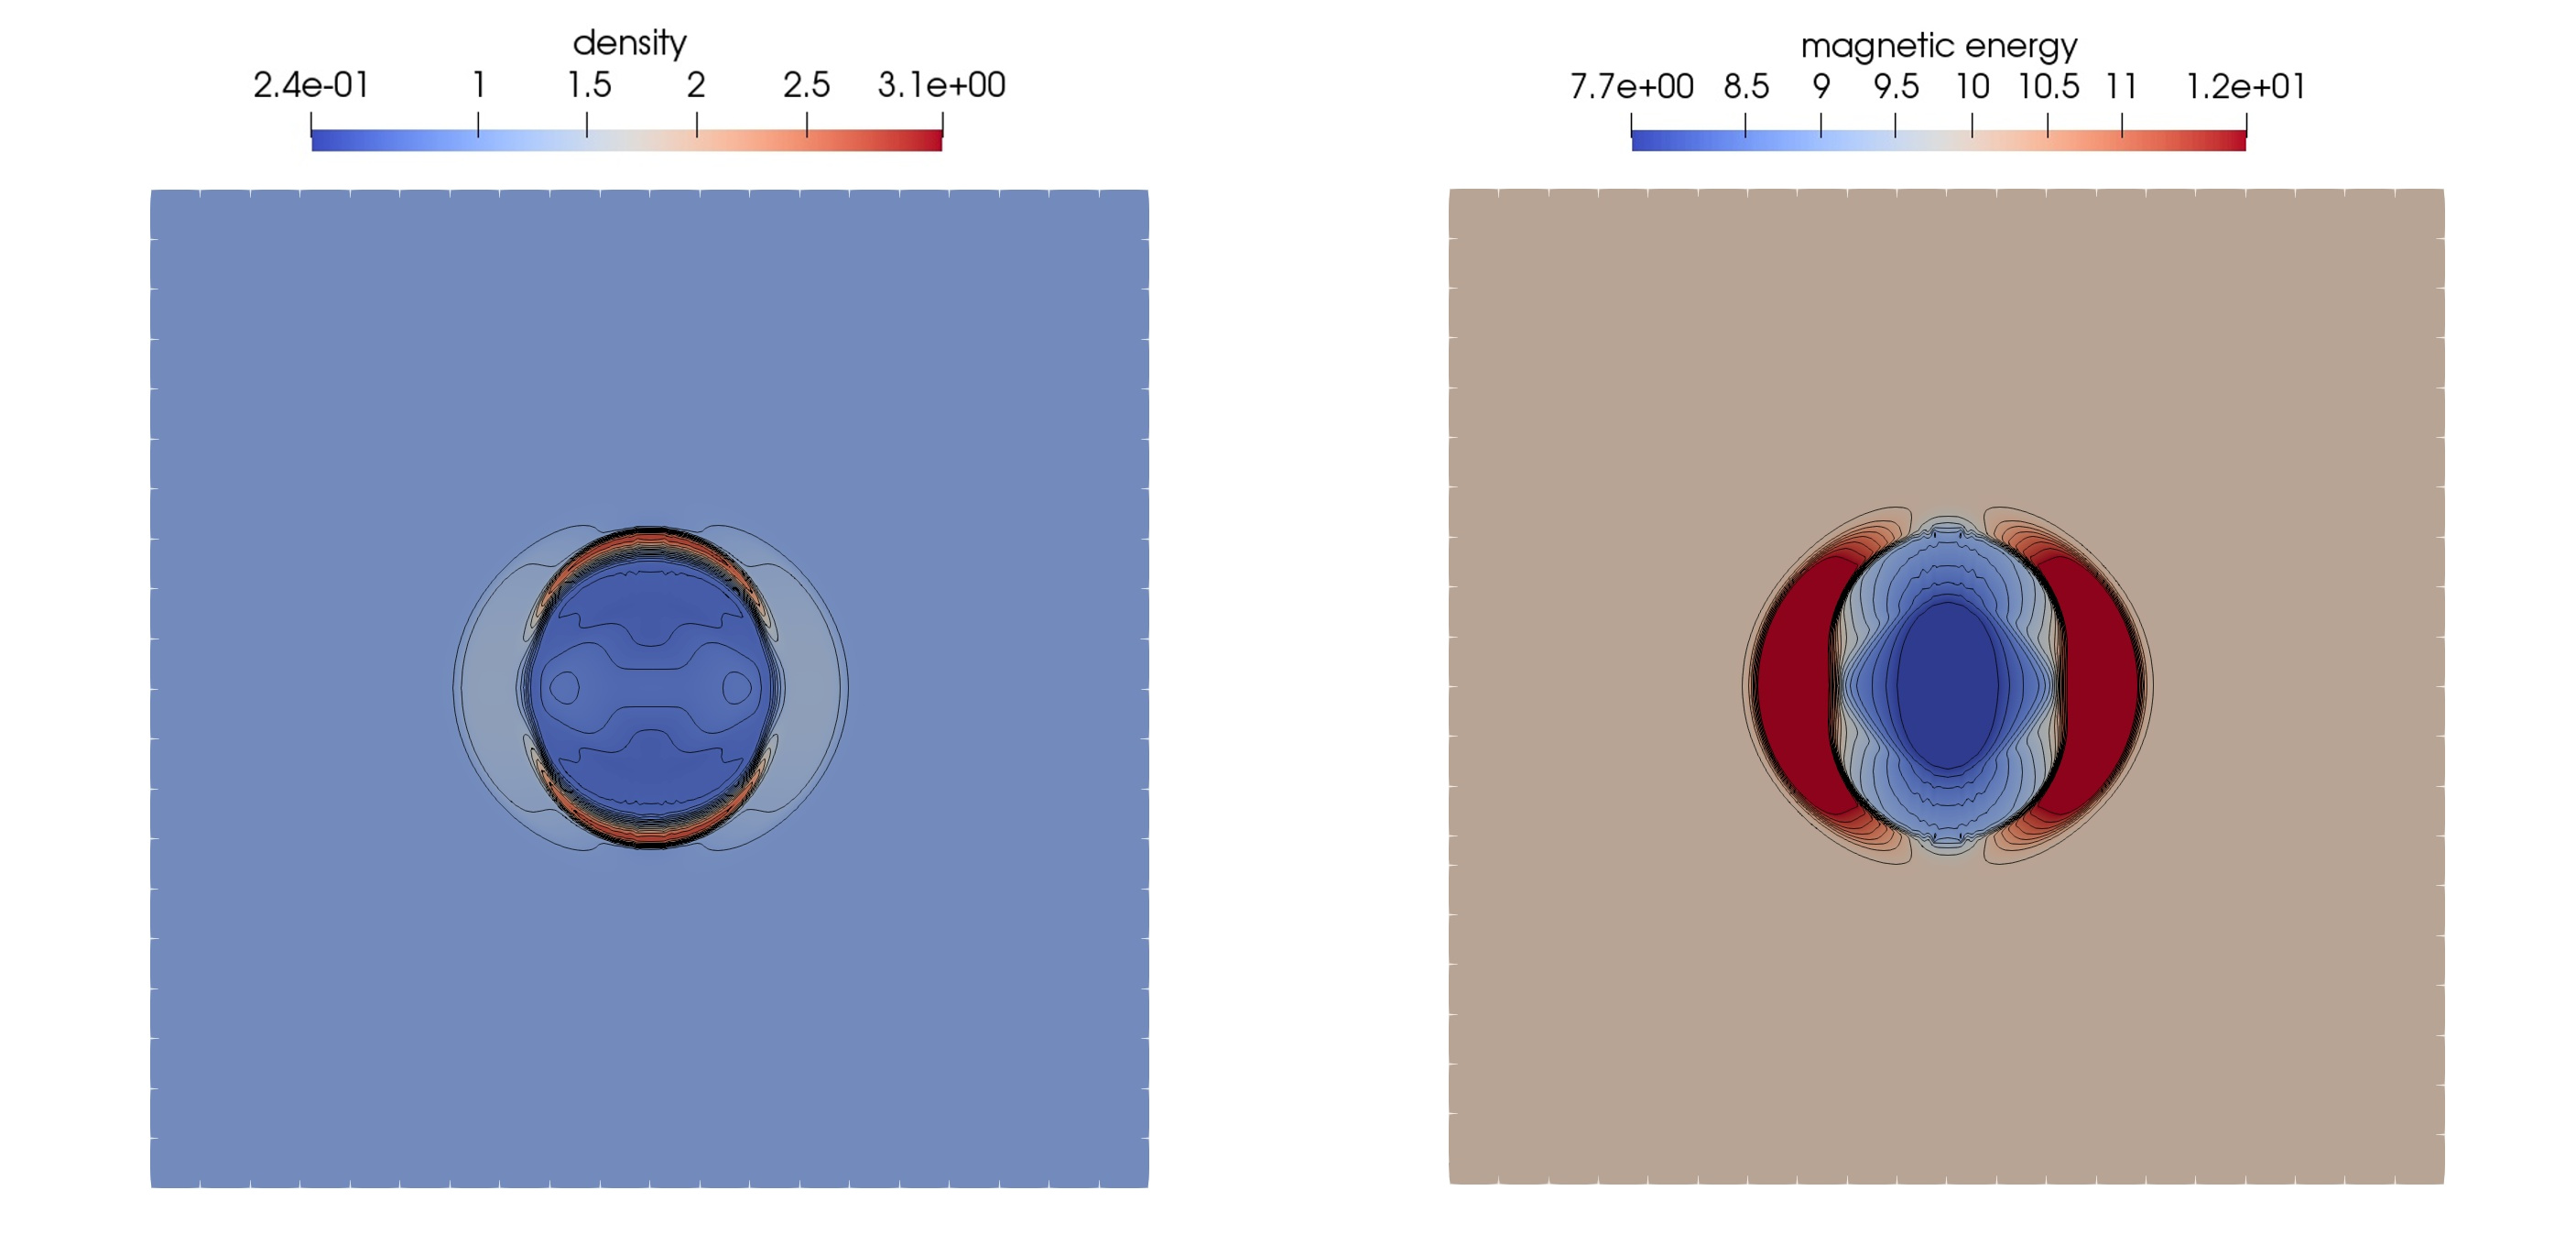
\includegraphics[width=0.87\textwidth]{img//mhd-blast/old/mynew2.jpg}
	\caption{Obtained results, $t = 6\times 10^{-3}$, density(left), magnetic energy(right)}
	\label{figure:blastOldMy2}
	\end{center}
\end{figure}
\vspace{-8mm}

\begin{figure}[H]
	\begin{center}
		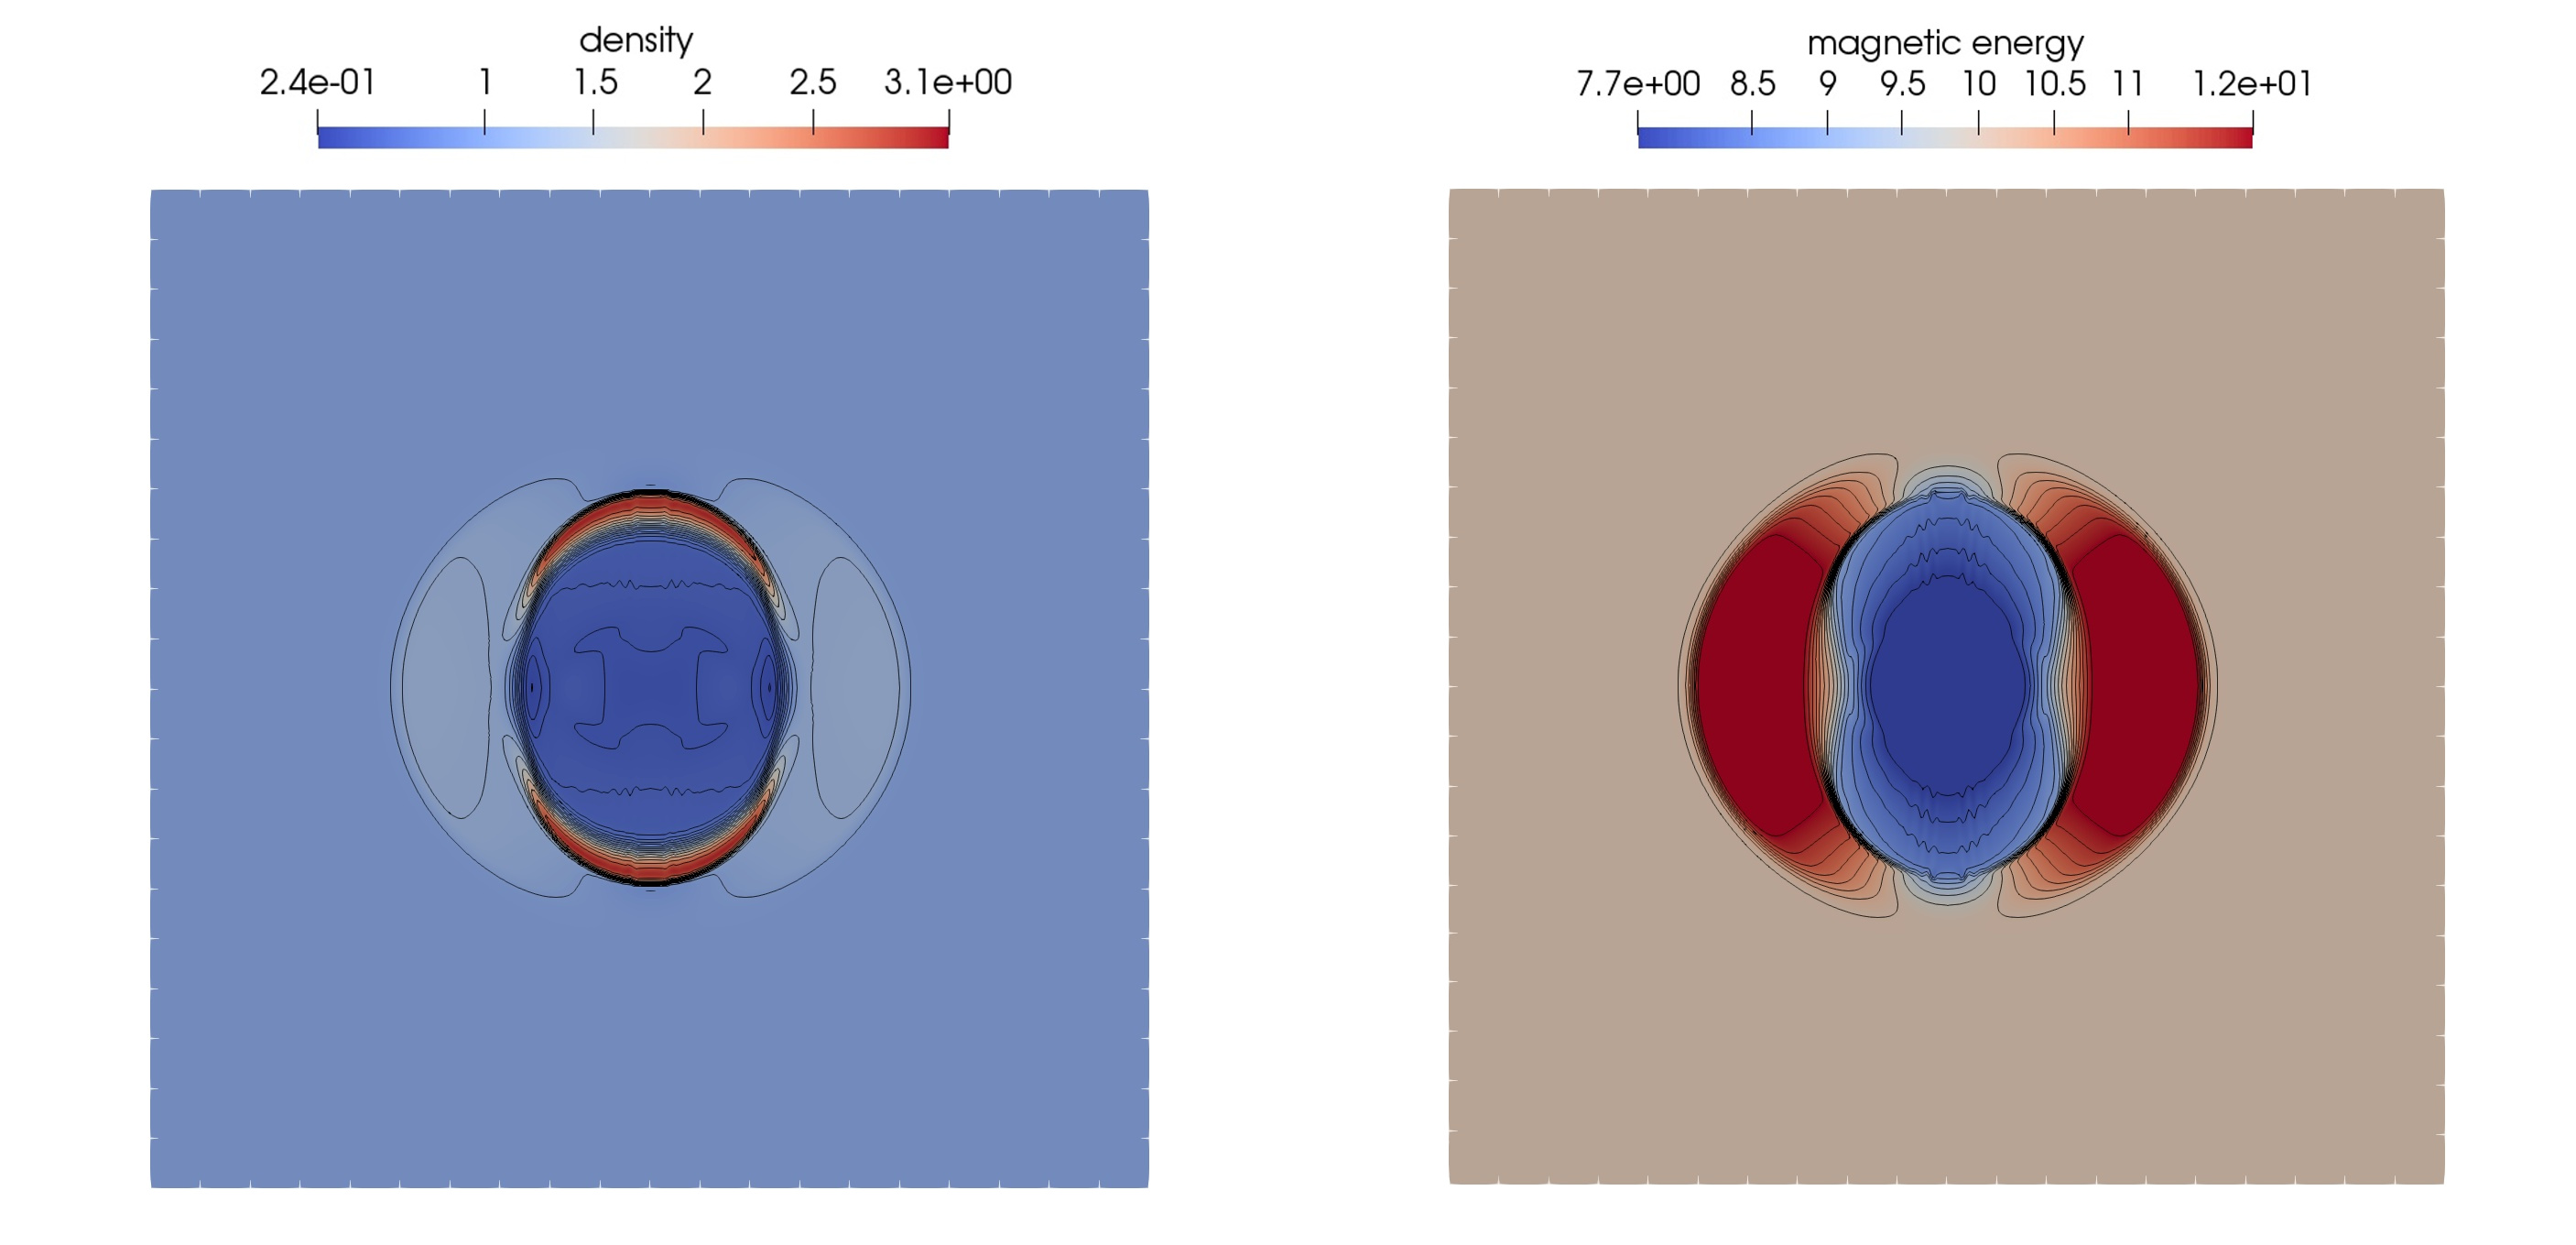
\includegraphics[width=0.87\textwidth]{img//mhd-blast/old/mynew3.jpg}
	\caption{Obtained results, $t = 11\times 10^{-3}$, density(left), magnetic energy(right)}
	\label{figure:blastOldMy3}
	\end{center}
\end{figure}
\vspace{-8mm}

\begin{figure}[H]
	\begin{center}
		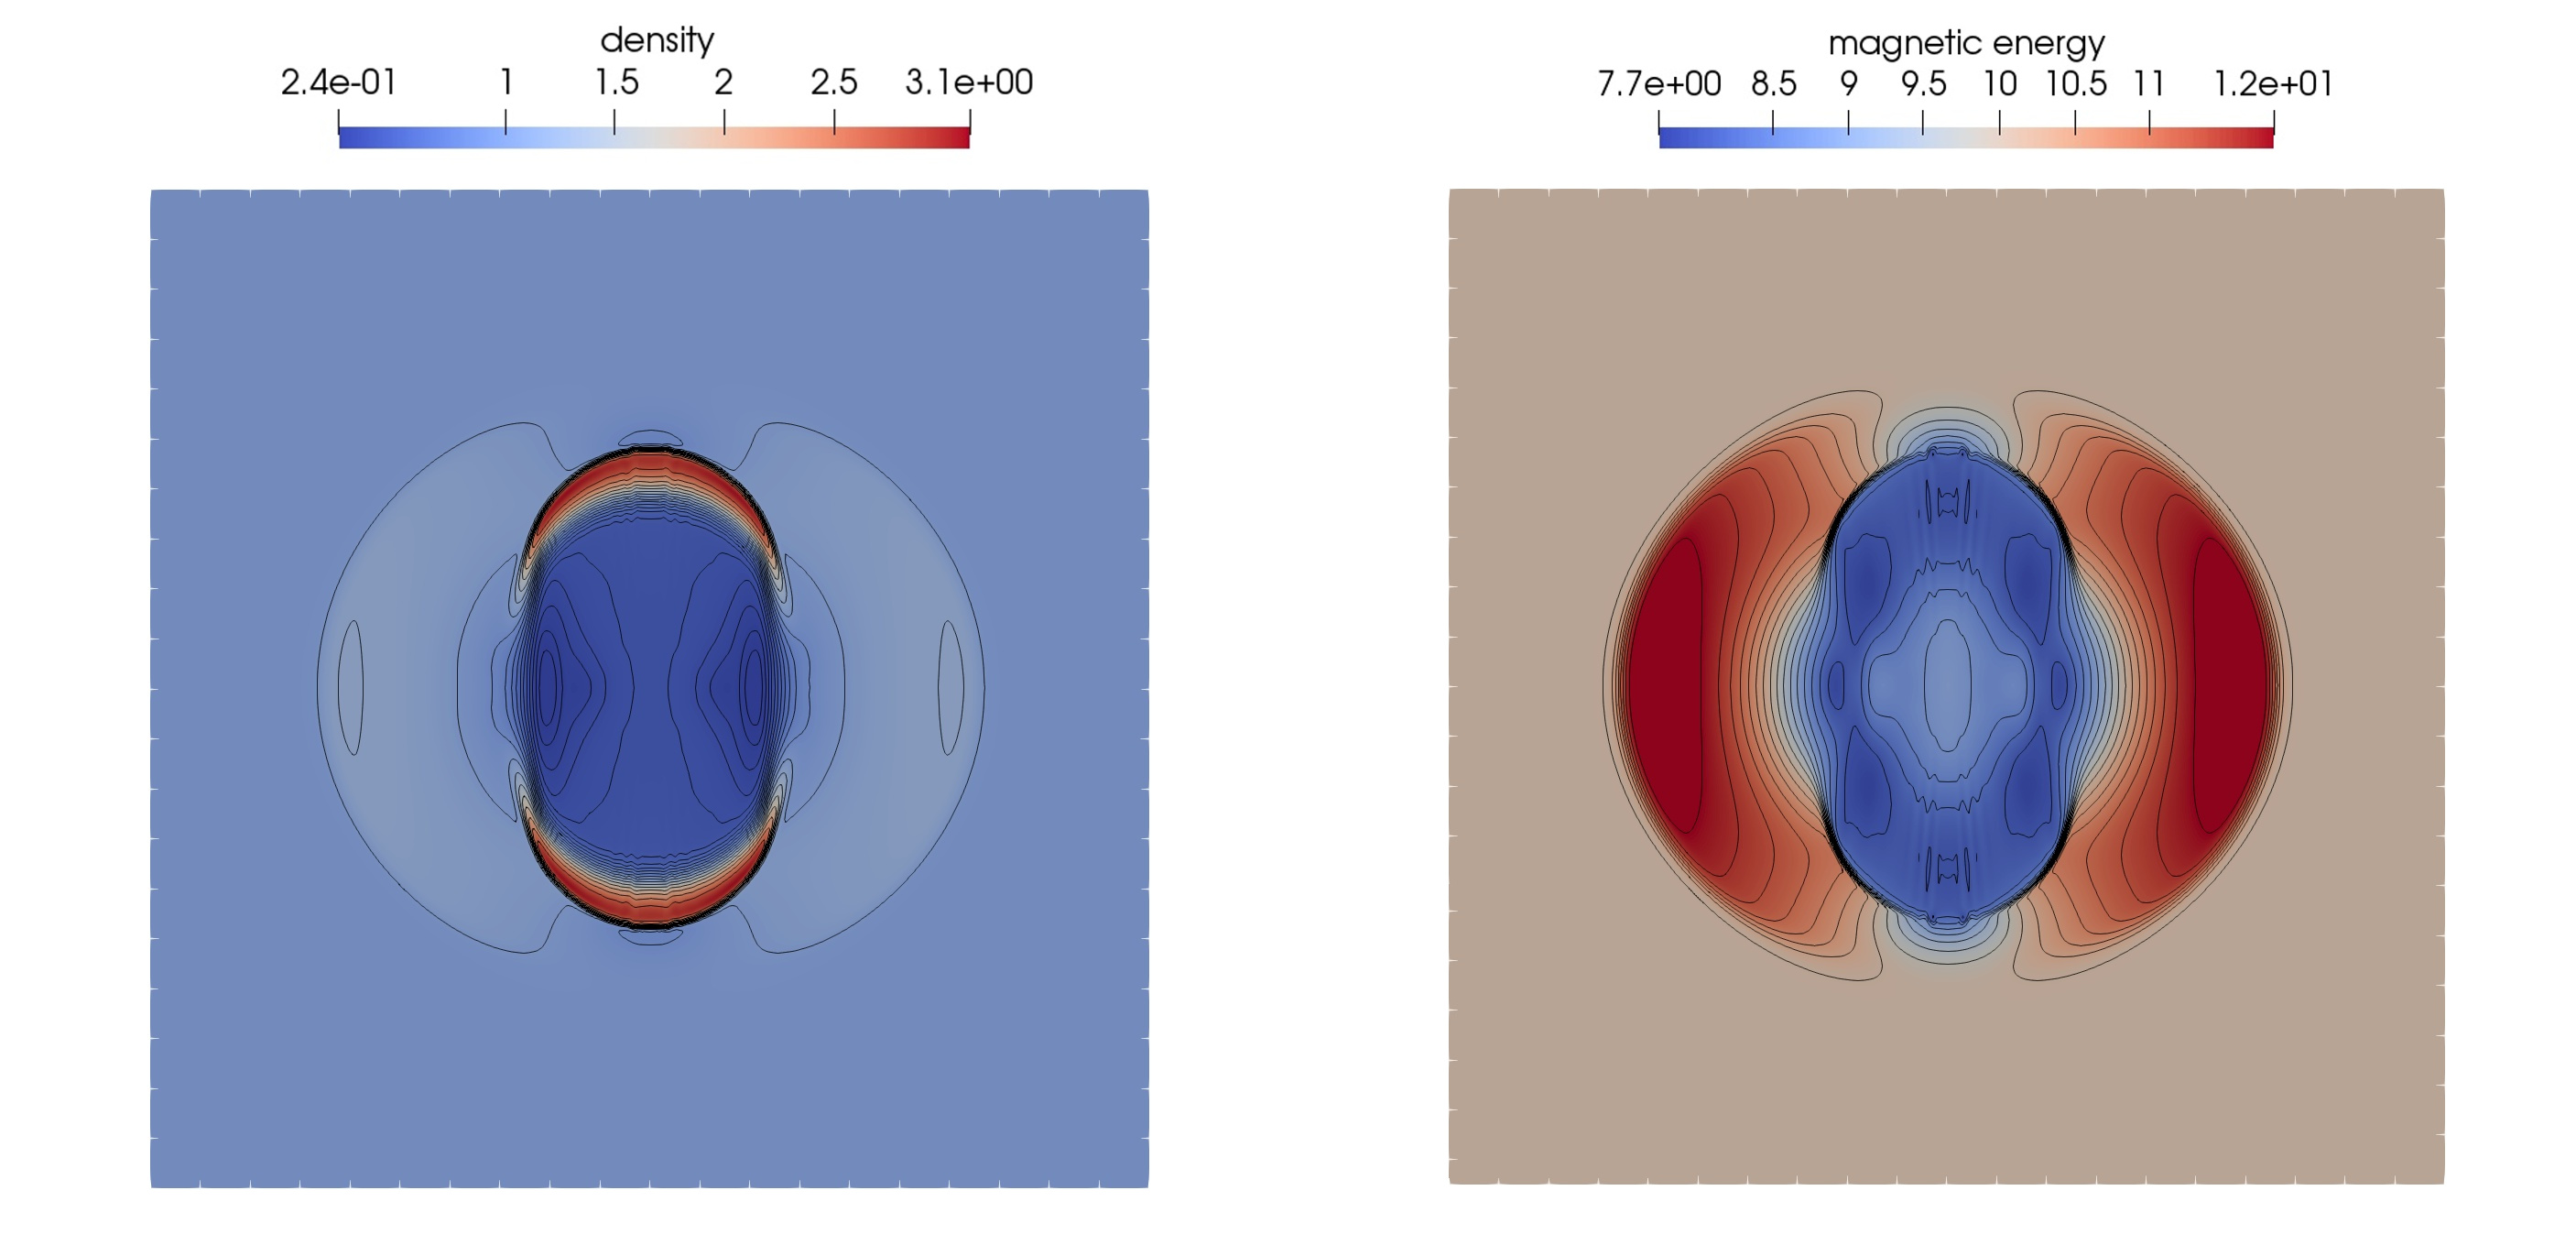
\includegraphics[width=0.87\textwidth]{img//mhd-blast/old/mynew4.jpg}
	\caption{Obtained results, $t = 16\times 10^{-3}$, density(left), magnetic energy(right)}
	\label{figure:blastOldMy4}
	\end{center}
\end{figure}
\vspace{-8mm}

\begin{figure}[H]
	\begin{center}
		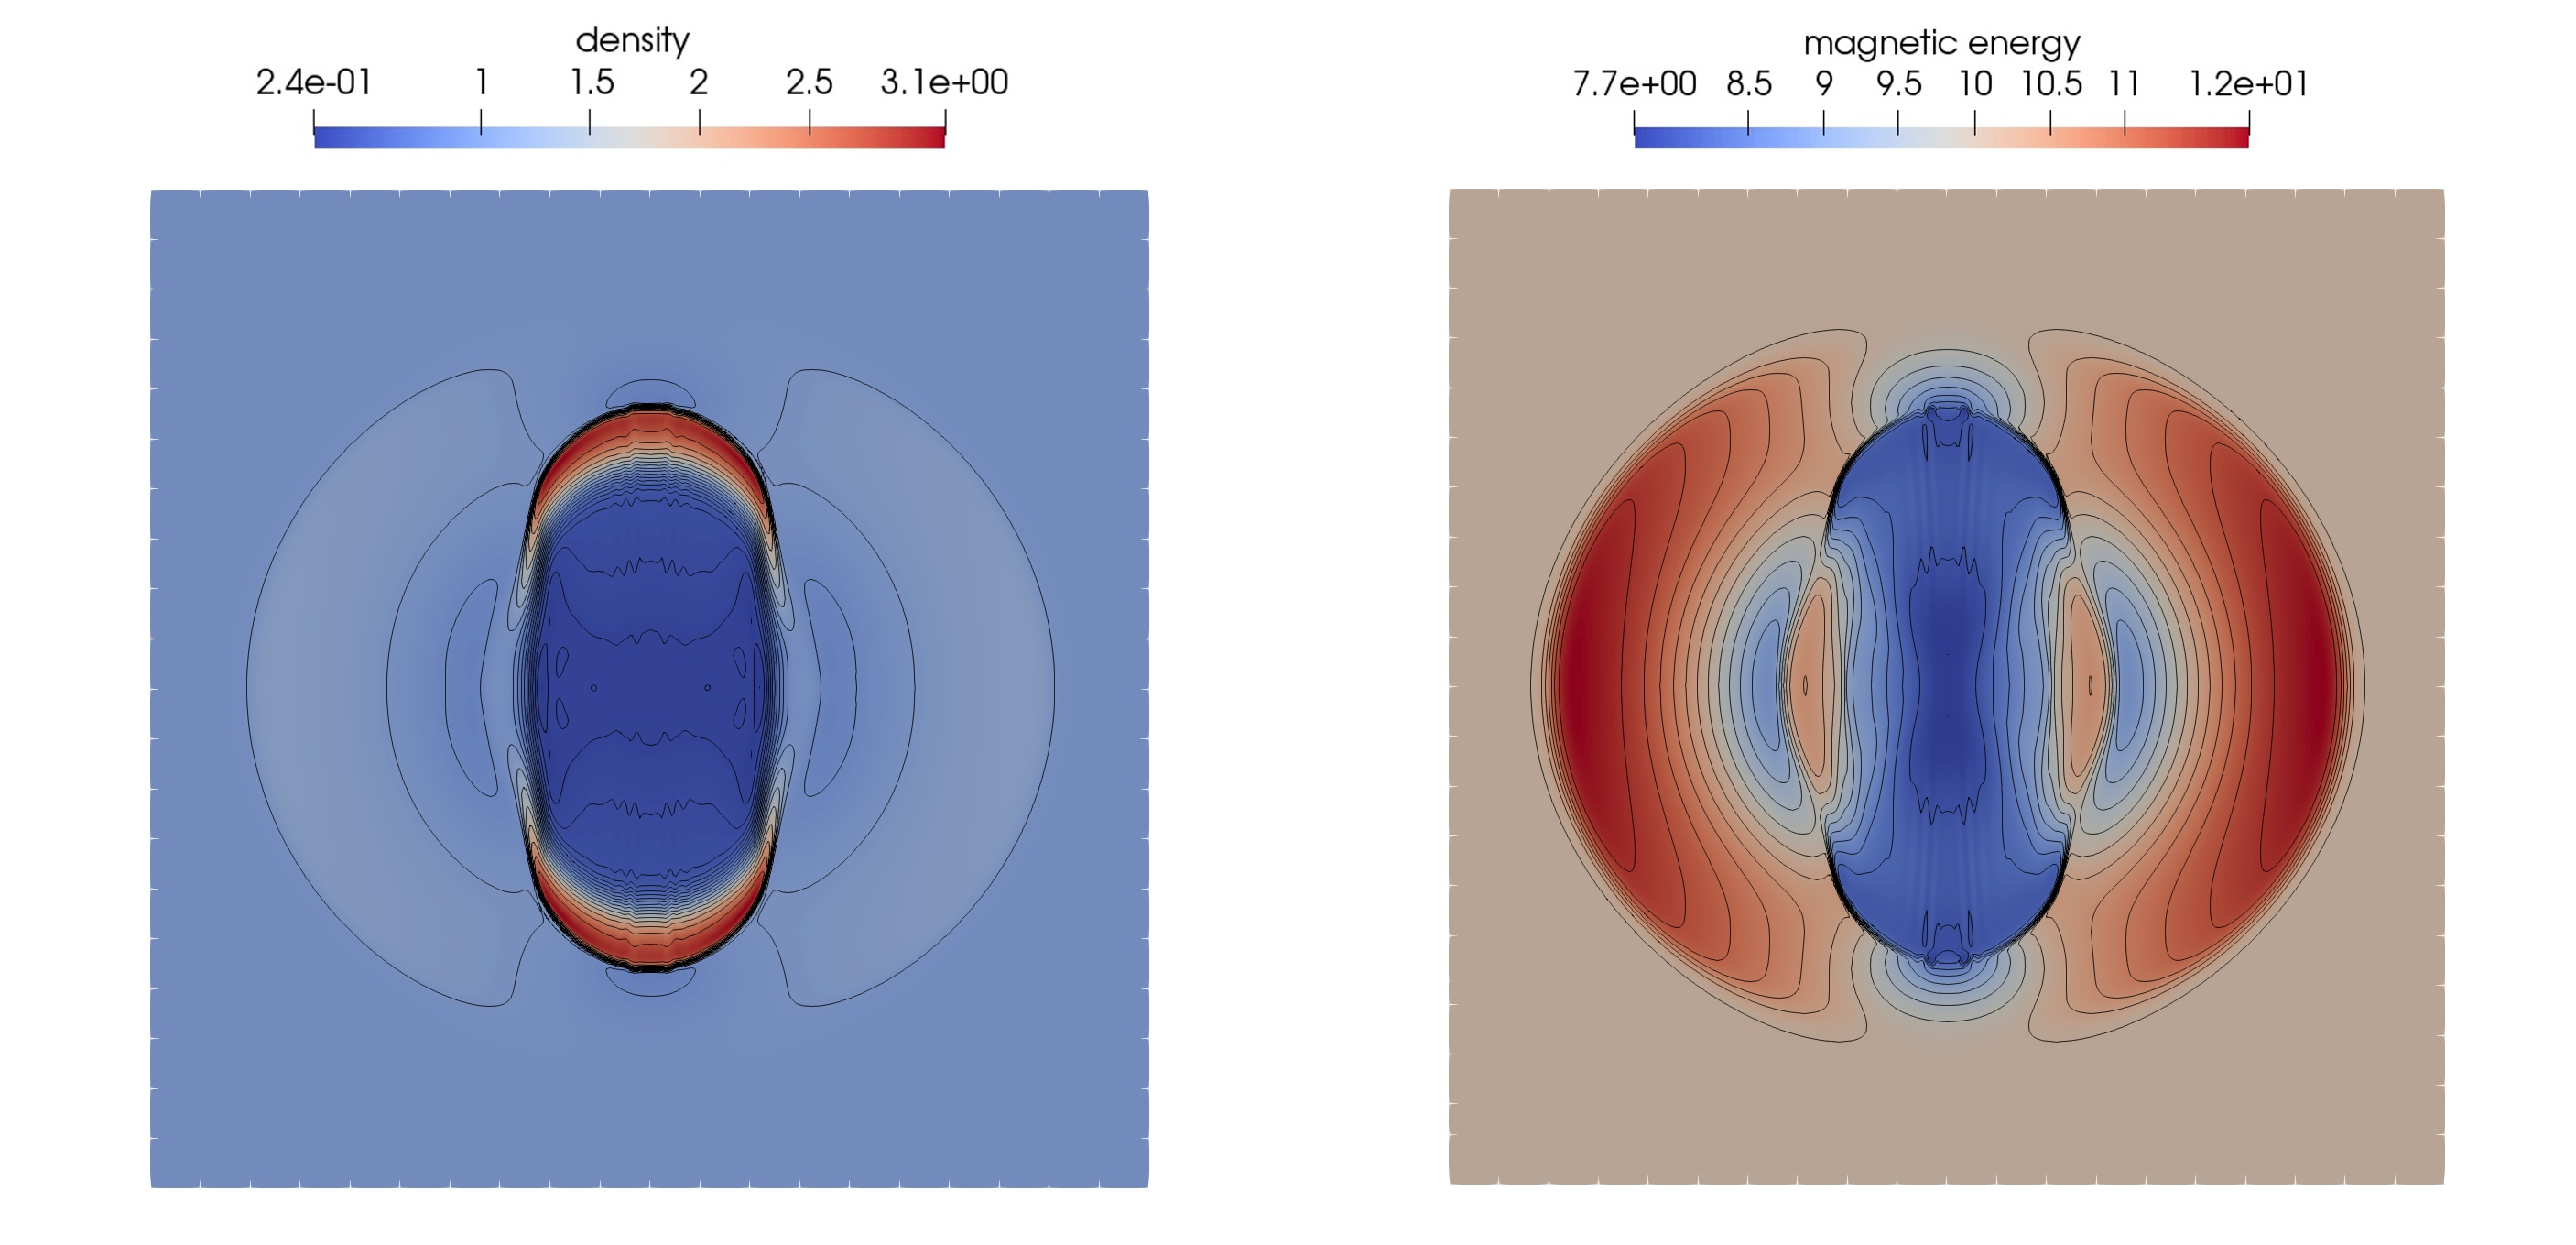
\includegraphics[width=0.87\textwidth]{img//mhd-blast/old/mynew5.jpg}
	\caption{Obtained results, $t = 23\times 10^{-3}$, density(left), magnetic energy(right)}
	\label{figure:blastOldMy5}
	\end{center}
\end{figure}
\vspace{-5mm}
The solution in \Cref{figure:blastOldMy4}, \Cref{figure:blastOldMy5}  is apparently almost identical to that in \Cref{figure:blastOldRef}. To demonstrate the distributed nature of the computation, in \Cref{figure:subdomainsBlastOld}, color-mapping of elements $K \in T$ to processors owning the particular element is presented (see \Cref{section:ditributedTria} for details). Note that there were $48$ processors used for the computation.

\begin{figure}[H]
	\begin{center}
		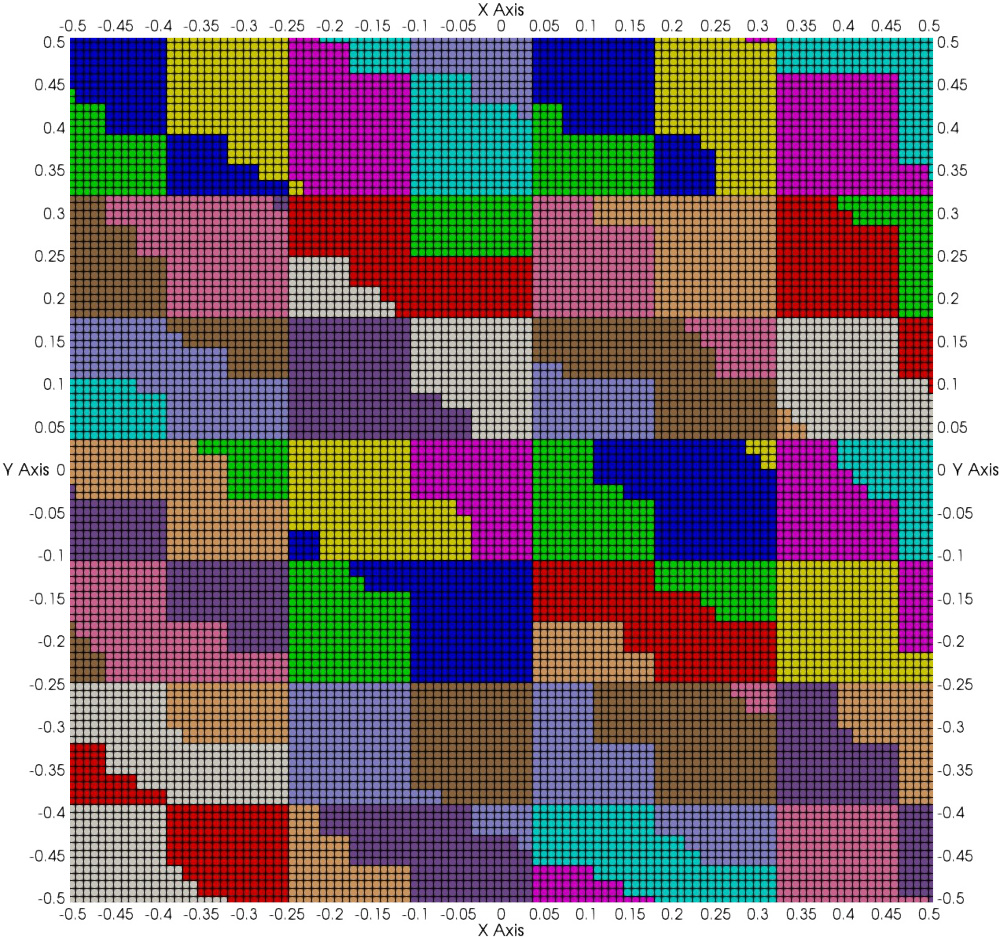
\includegraphics[width=0.5\textwidth]{img//mhd-blast/old/subdomain.jpg}
	\caption{Color-mapping of elements to processors for the computation of \Crefrange{figure:blastOldMy1}{figure:blastOldMy5}}
	\label{figure:subdomainsBlastOld}
	\end{center}
\end{figure}
\vspace{-5mm}

This however, was a static calculation with 200 mesh elements in the $x-$ and $y-$ dimensions. In order to see how the AMR (see \Cref{chapter:amr}) performs, the same computation was performed in adaptive setup. Starting from a very coarse mesh of 10 elements in both dimensions, the evolving mesh and its distribution to processors are shown in \Crefrange{figure:blastOldMyAdapt1}{figure:blastOldMyAdapt6} - the distribution to processors on the left, the mesh elements on the right.

\begin{figure}[H]
	\begin{center}
		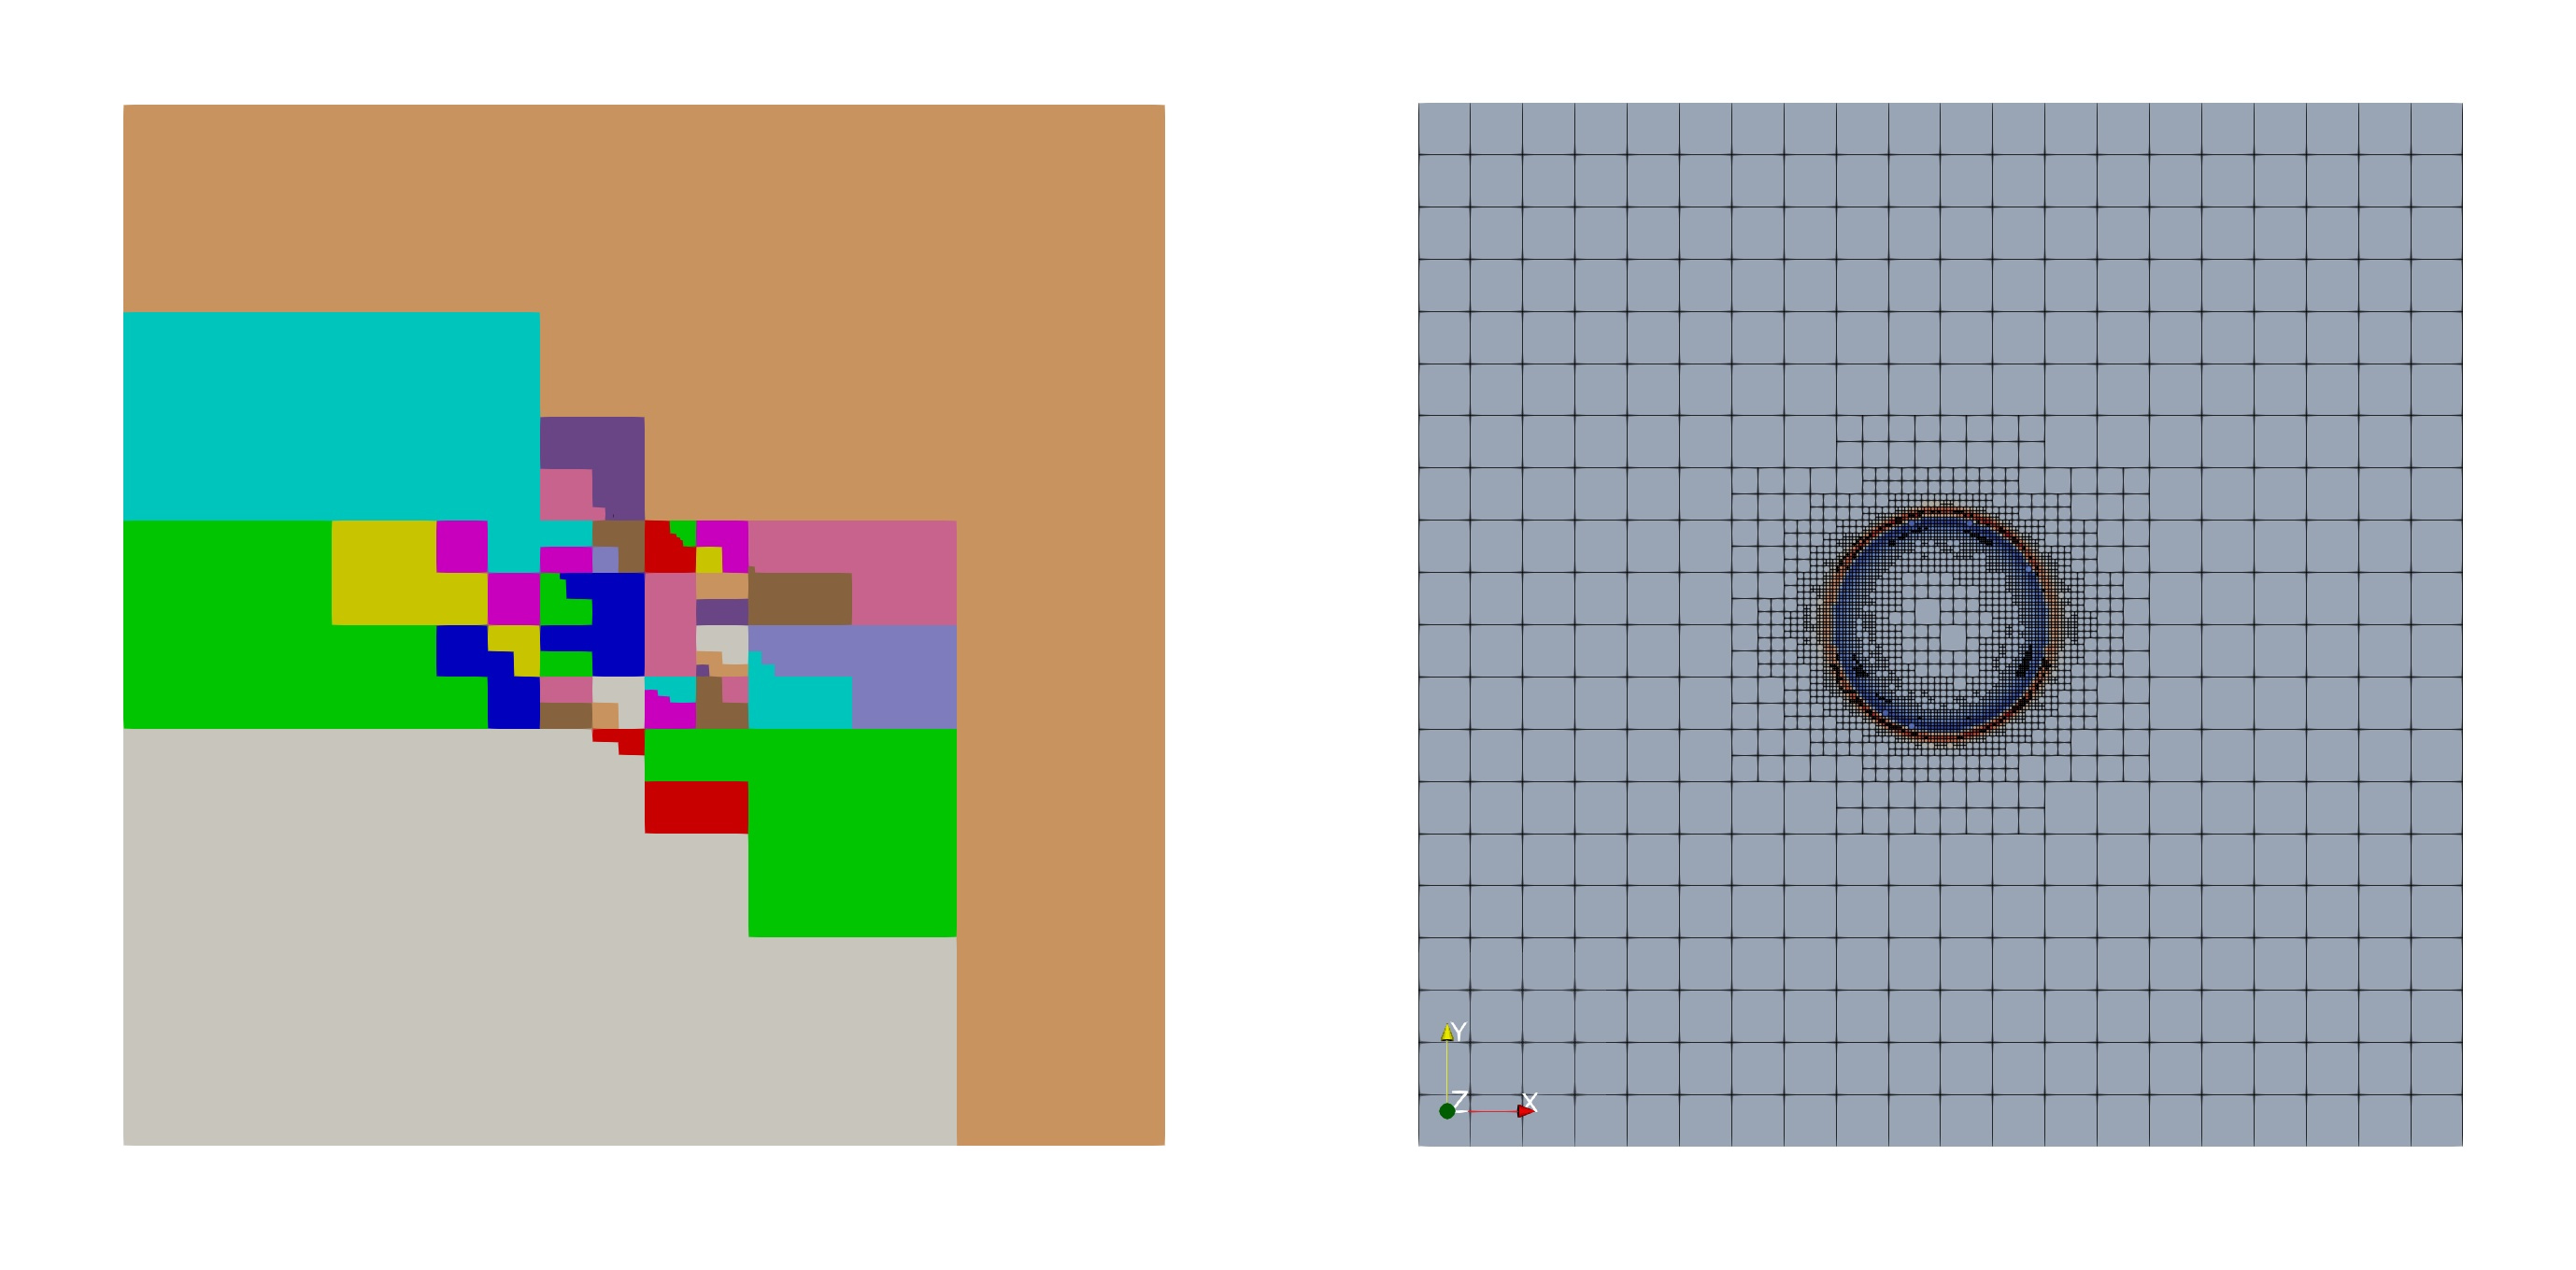
\includegraphics[width=0.87\textwidth]{img//mhd-blast/old/mya1.jpg}
	\caption{Obtained results, initial state, distribution of elements (right) to processors (left)}
	\label{figure:blastOldMyAdapt1}
	\end{center}
\end{figure}
\vspace{-8mm}

\begin{figure}[H]
	\begin{center}
		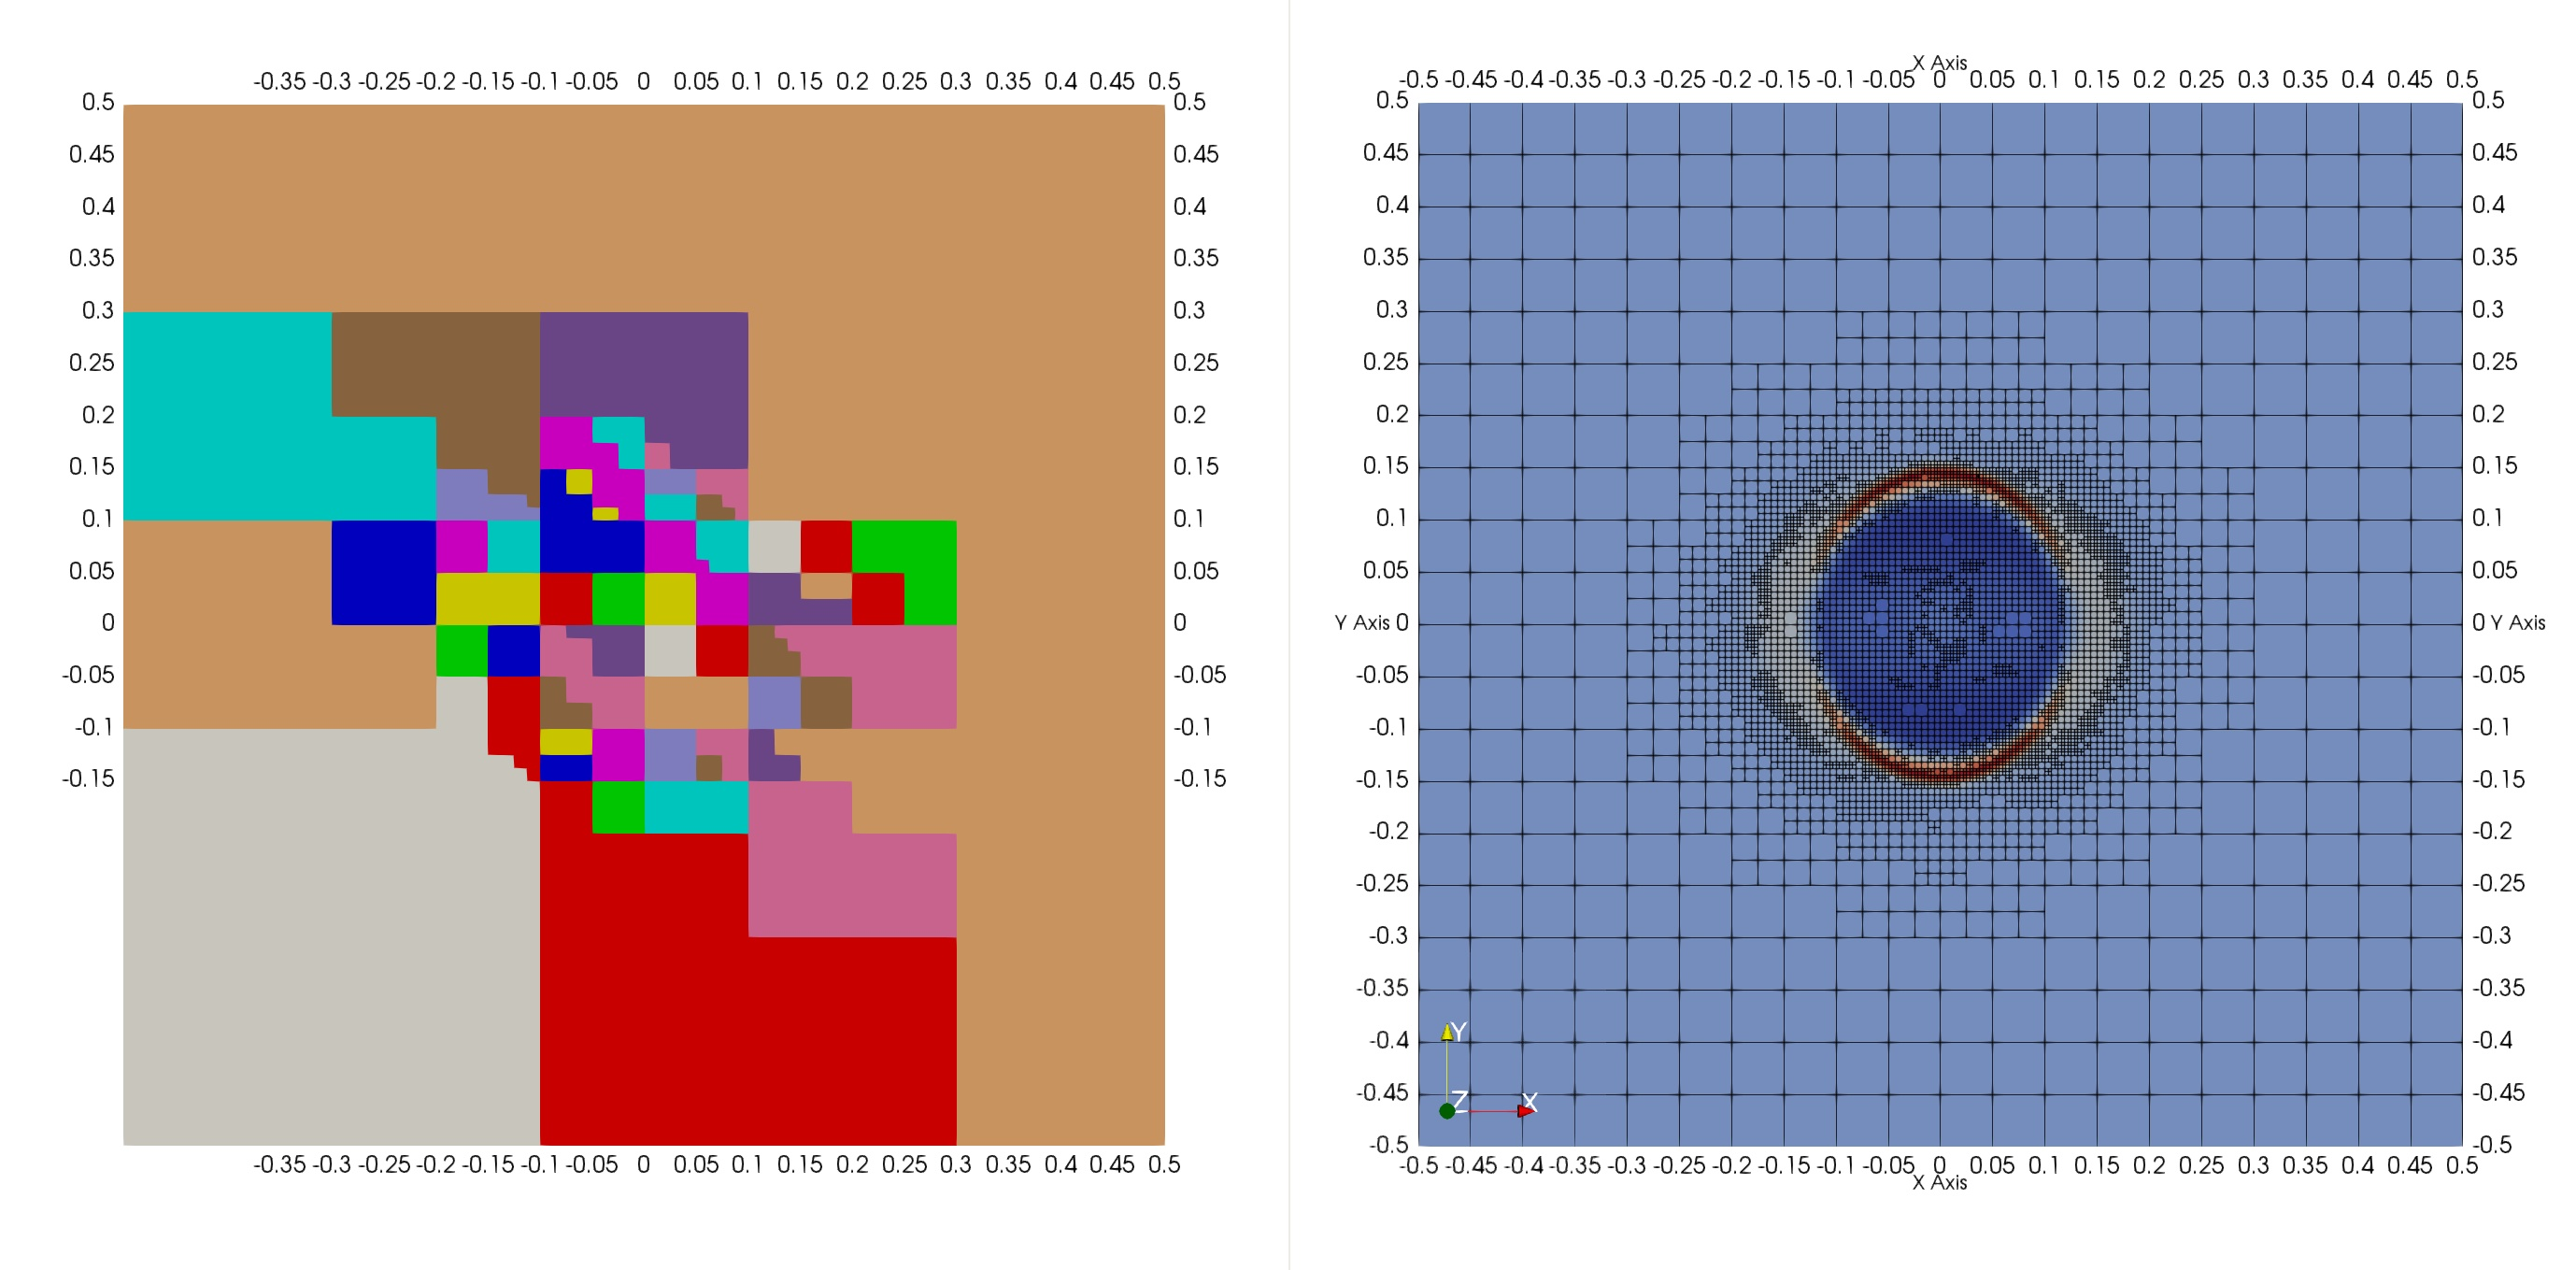
\includegraphics[width=0.87\textwidth]{img//mhd-blast/old/mya2.jpg}
	\caption{Obtained results, $t = 5\times 10^{-3}$, distribution of elements (right) to processors (left)}
	\label{figure:blastOldMyAdapt2}
	\end{center}
\end{figure}
\vspace{-8mm}

\begin{figure}[H]
	\begin{center}
		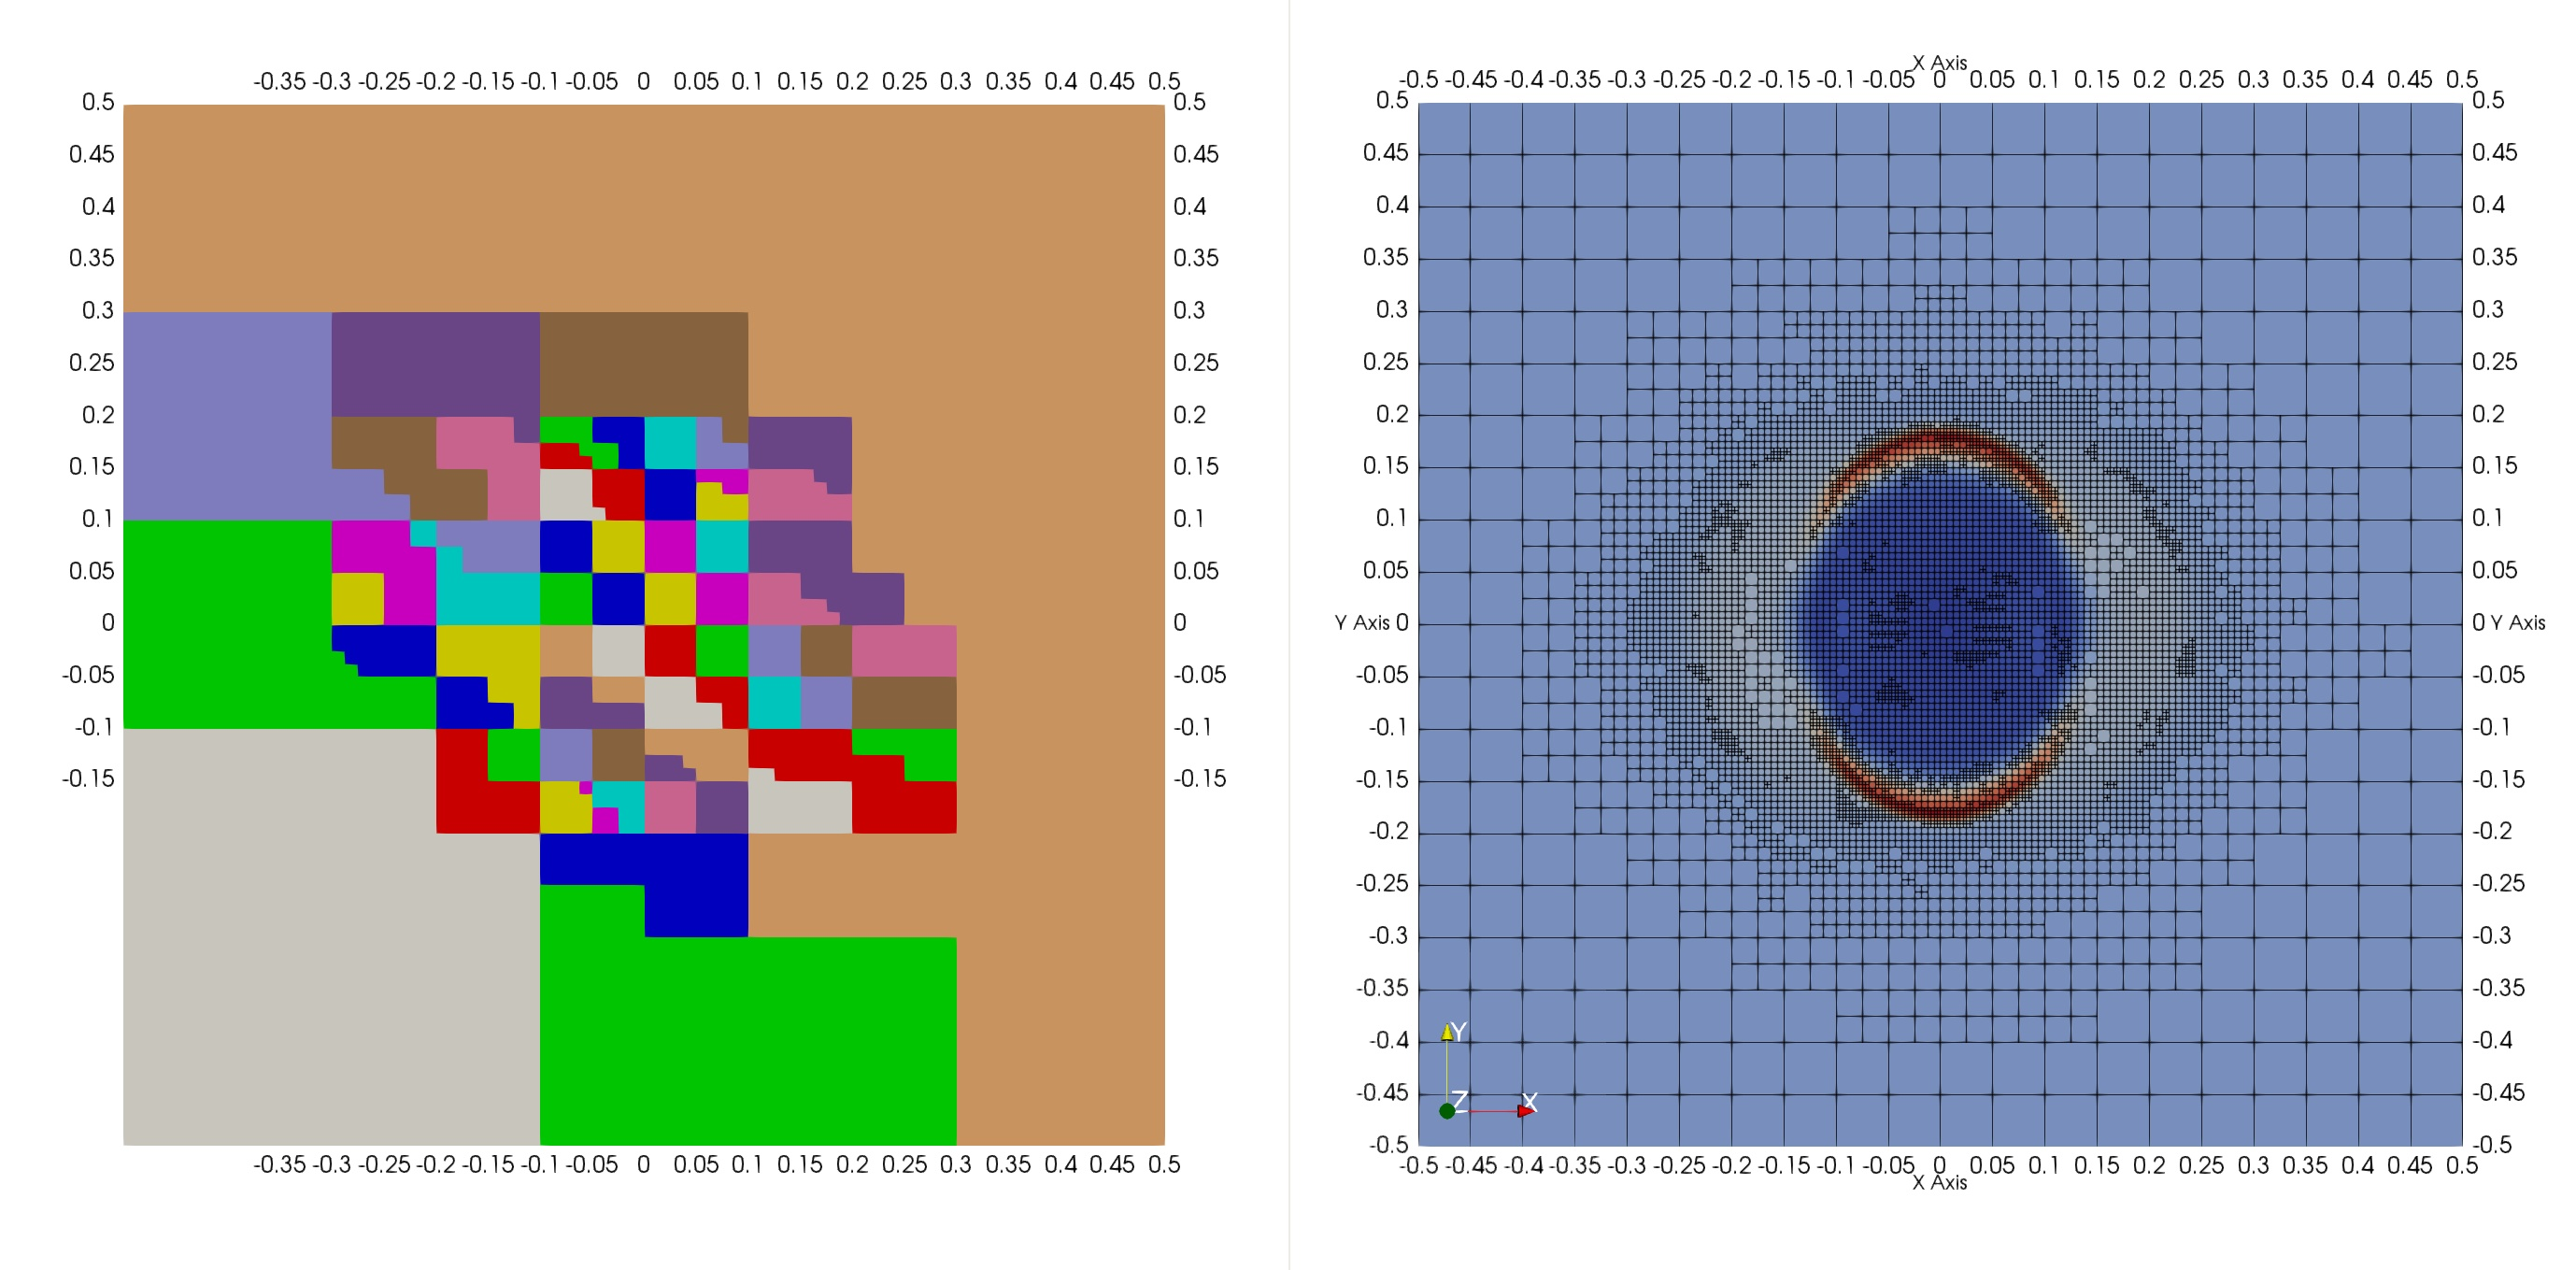
\includegraphics[width=0.87\textwidth]{img//mhd-blast/old/mya3.jpg}
	\caption{Obtained results, $t = 10\times 10^{-3}$, distribution of elements (right) to processors (left)}
	\label{figure:blastOldMyAdapt3}
	\end{center}
\end{figure}
\vspace{-8mm}

\begin{figure}[H]
	\begin{center}
		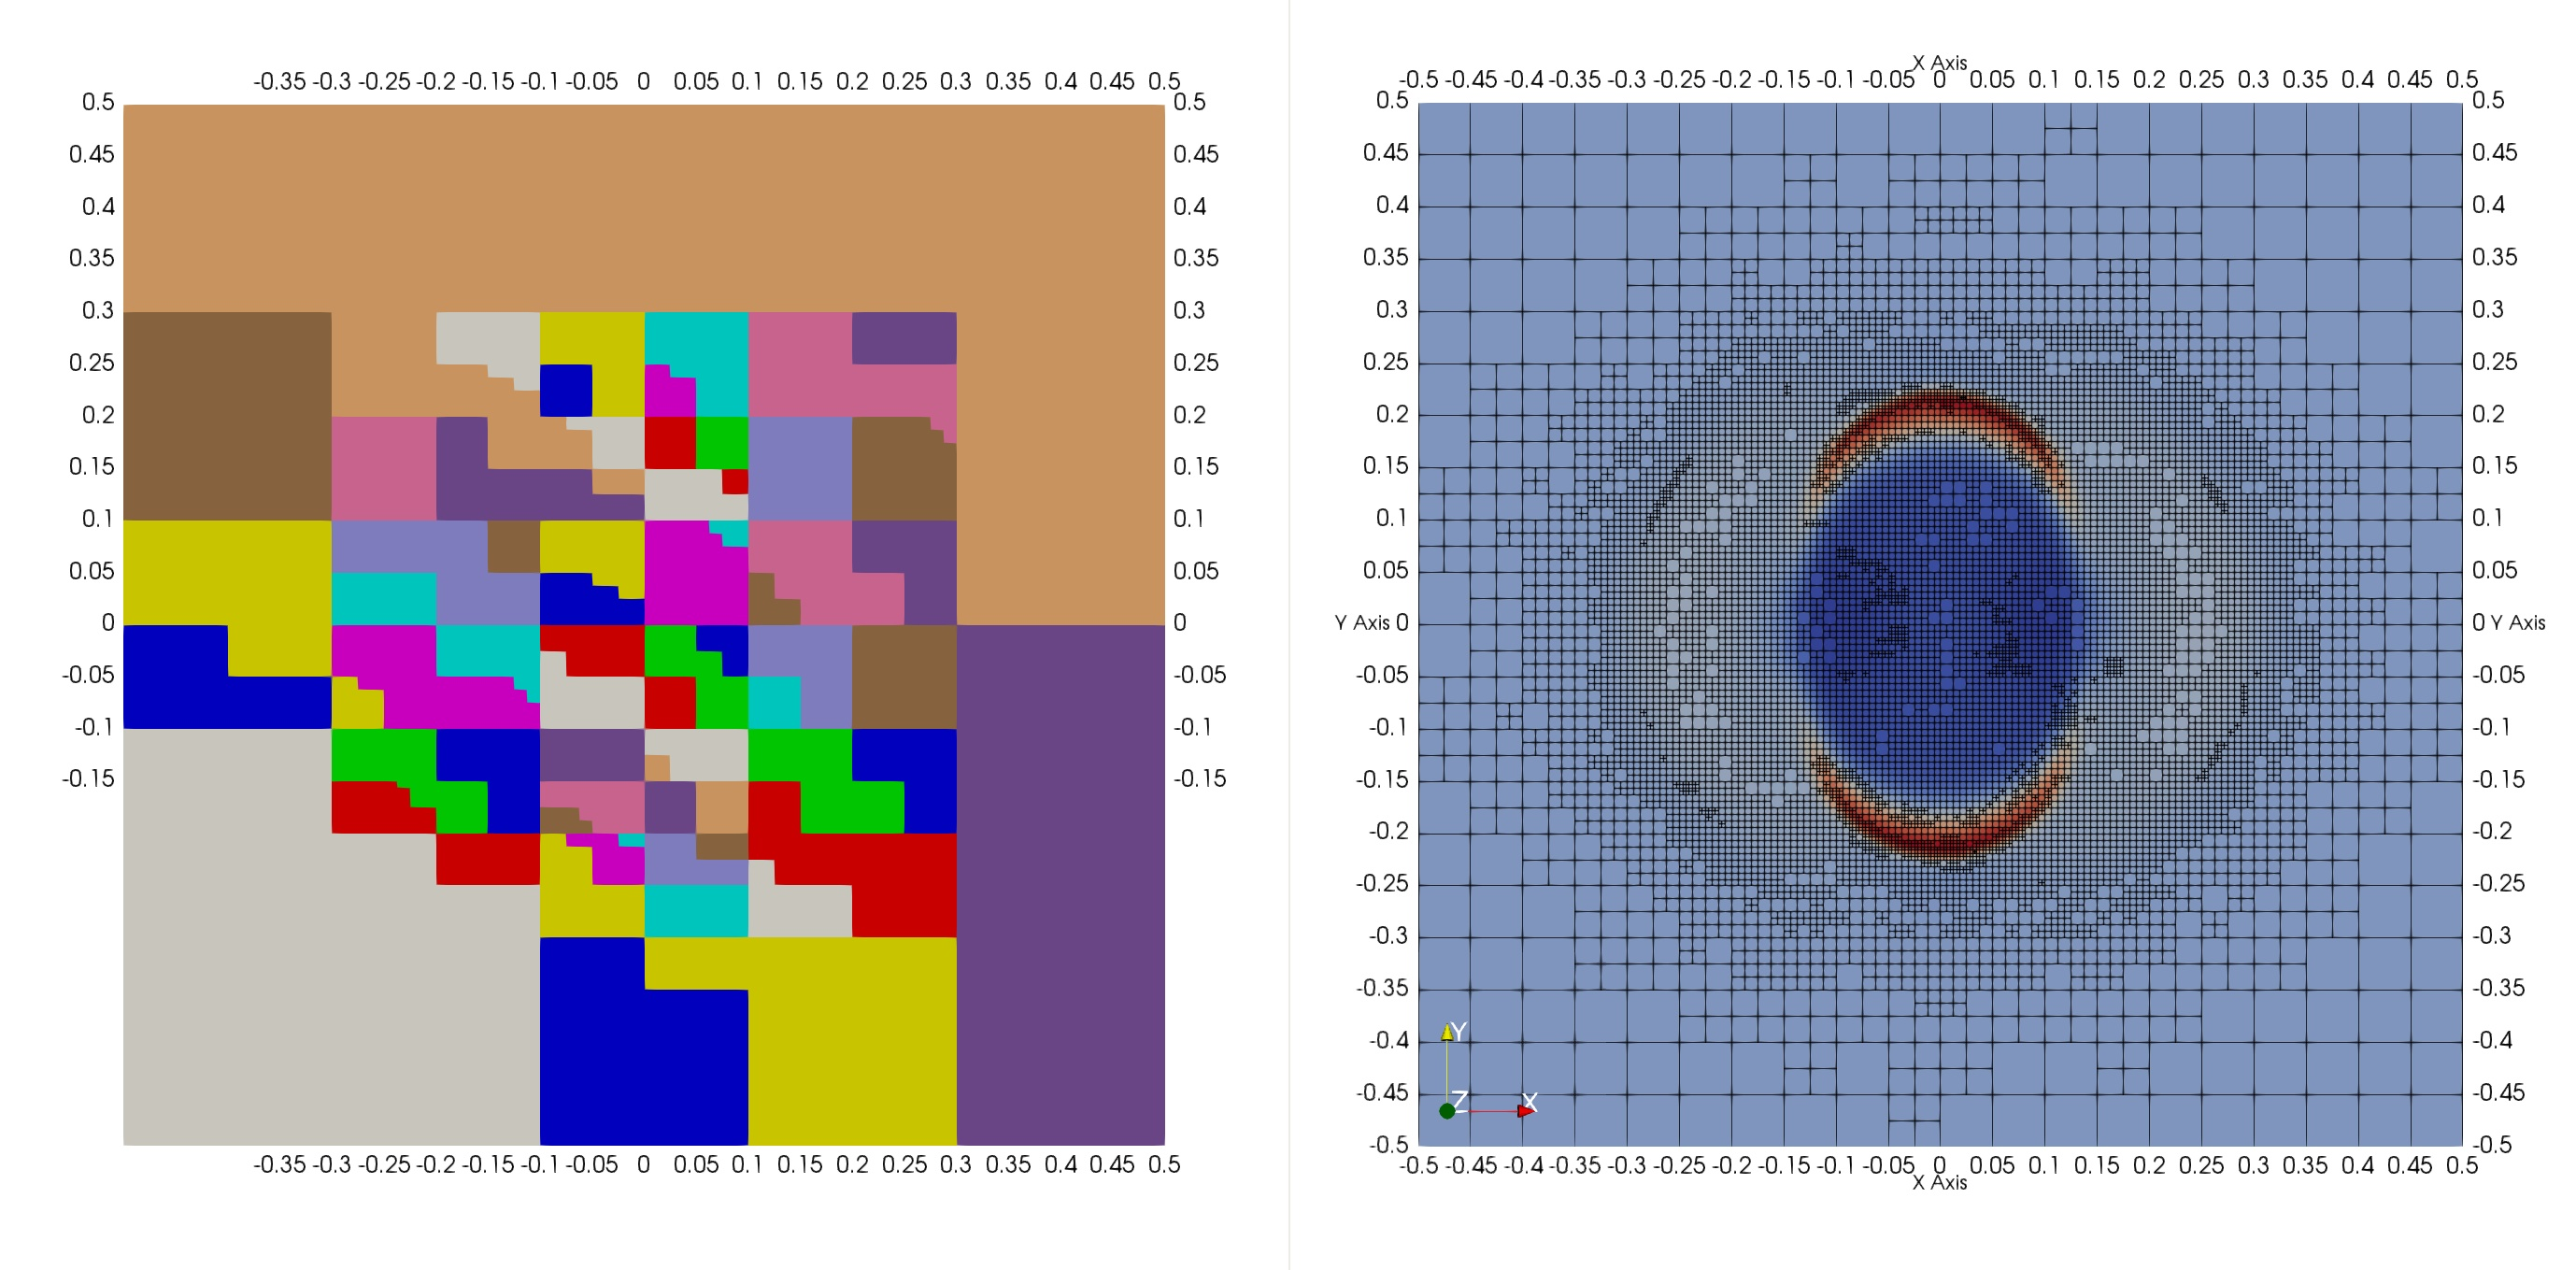
\includegraphics[width=0.87\textwidth]{img//mhd-blast/old/mya4.jpg}
	\caption{Obtained results, $t = 15\times 10^{-3}$, distribution of elements (right) to processors (left)}
	\label{figure:blastOldMyAdapt4}
	\end{center}
\end{figure}
\vspace{-8mm}

\begin{figure}[H]
	\begin{center}
		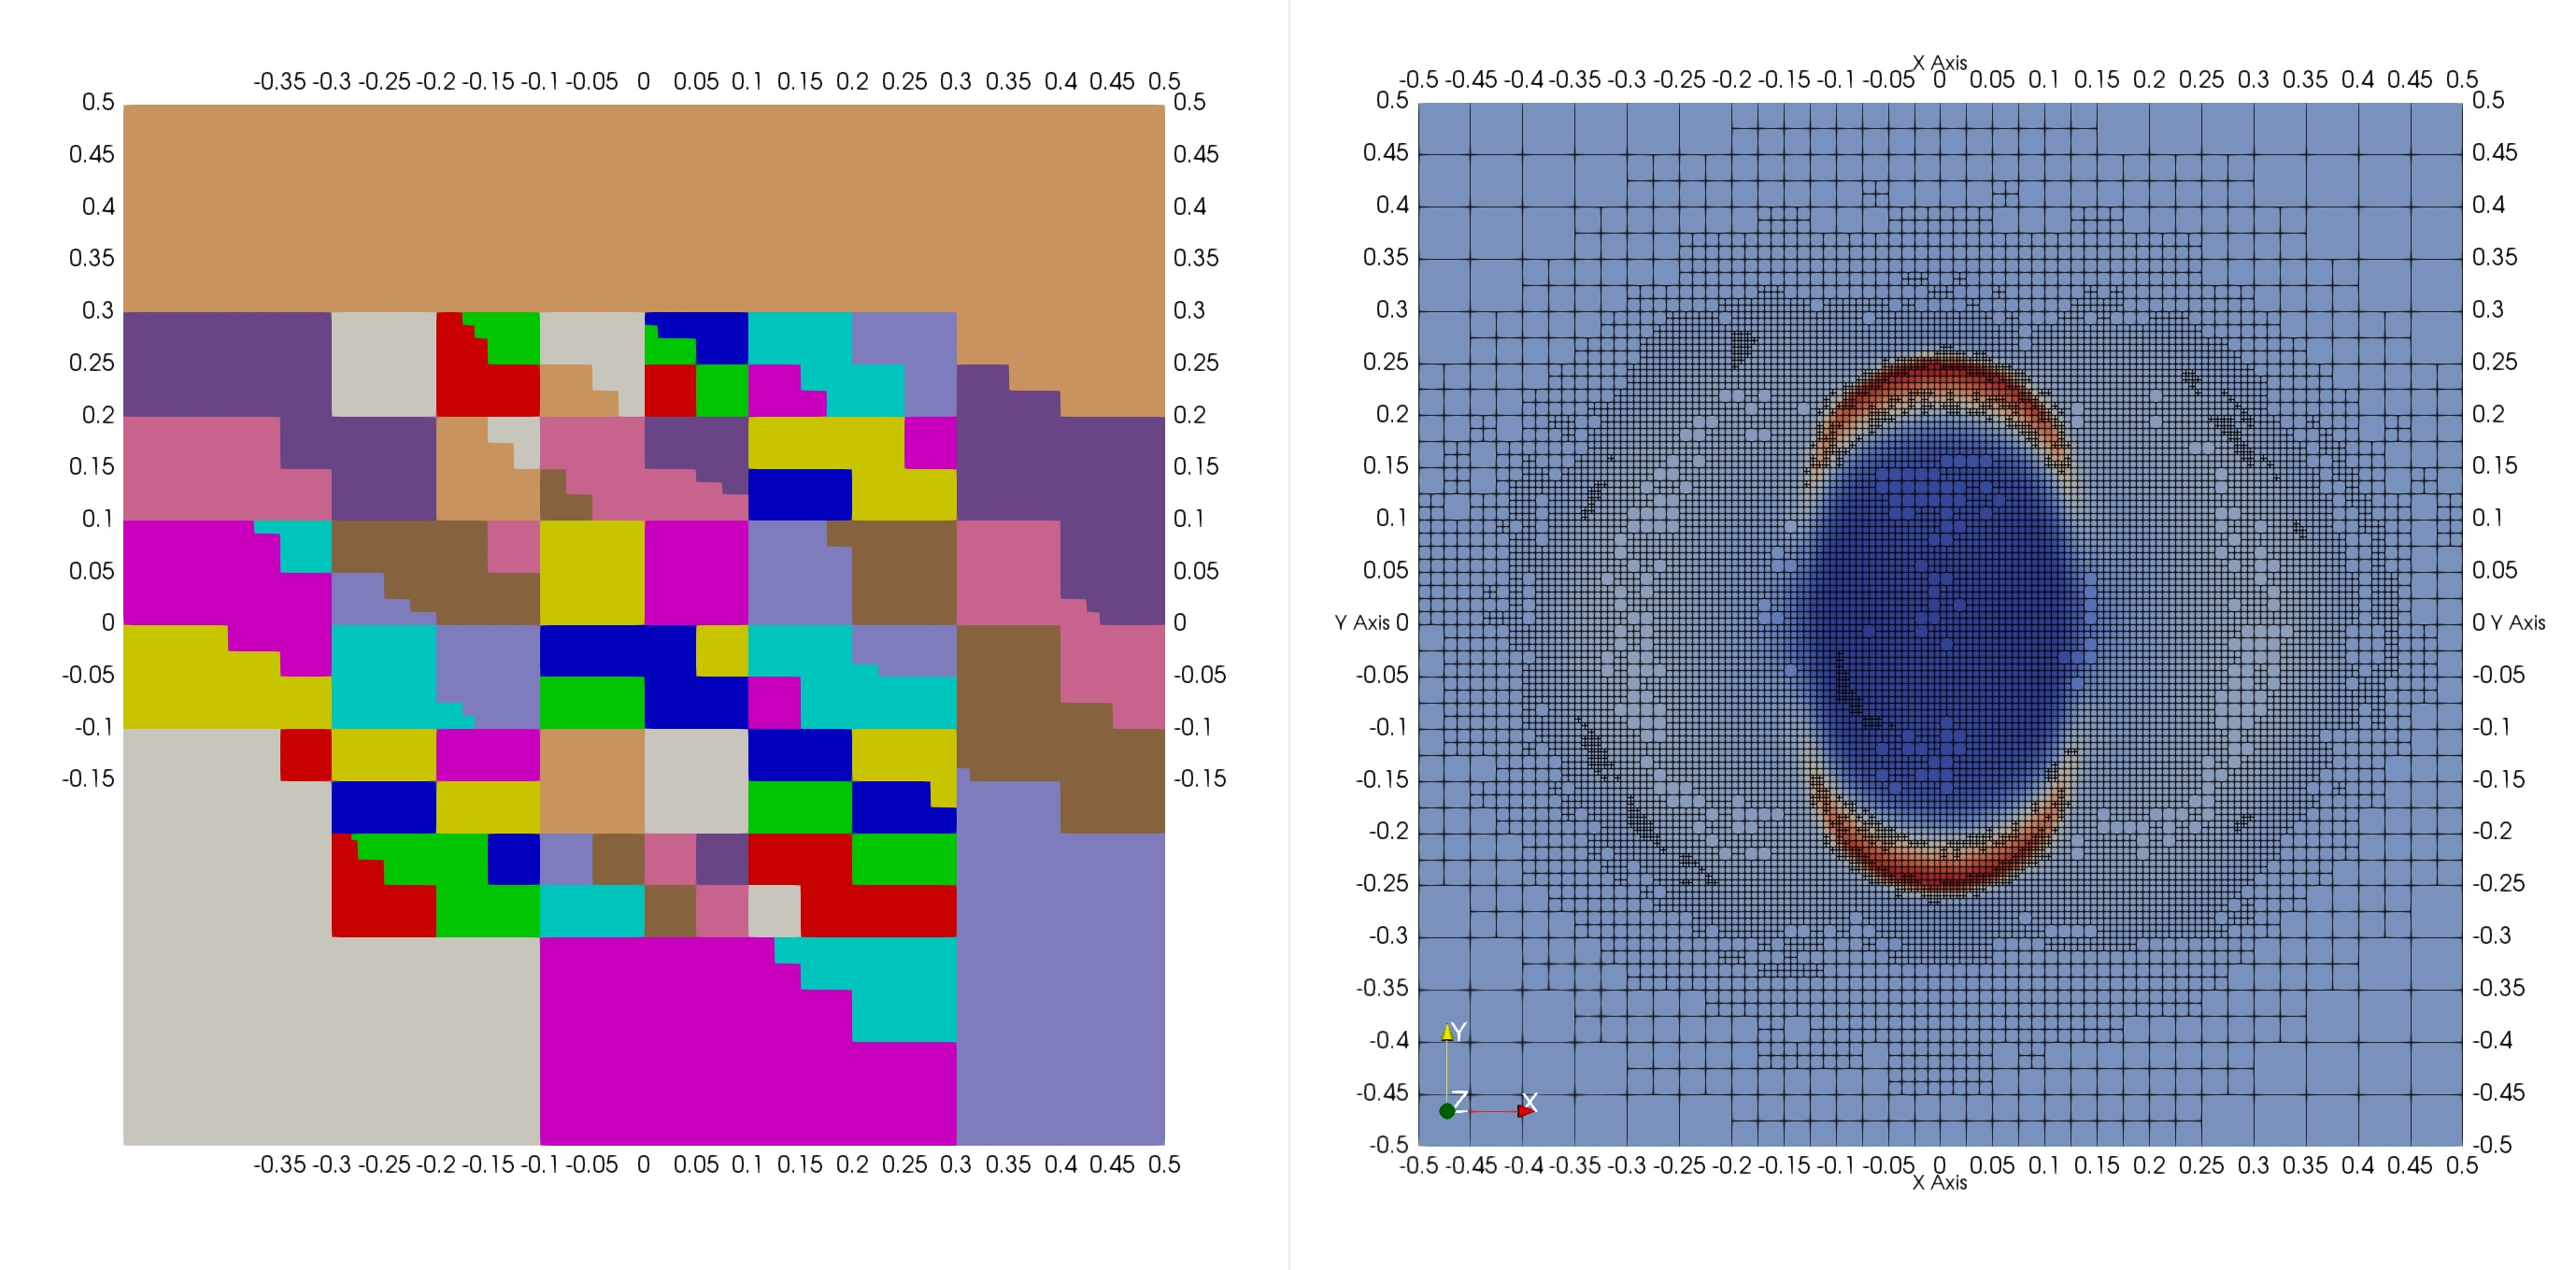
\includegraphics[width=0.87\textwidth]{img//mhd-blast/old/mya5.jpg}
	\caption{Obtained results, $t = 20\times 10^{-3}$, distribution of elements (right) to processors (left)}
	\label{figure:blastOldMyAdapt5}
	\end{center}
\end{figure}
\vspace{-8mm}

\begin{figure}[H]
	\begin{center}
		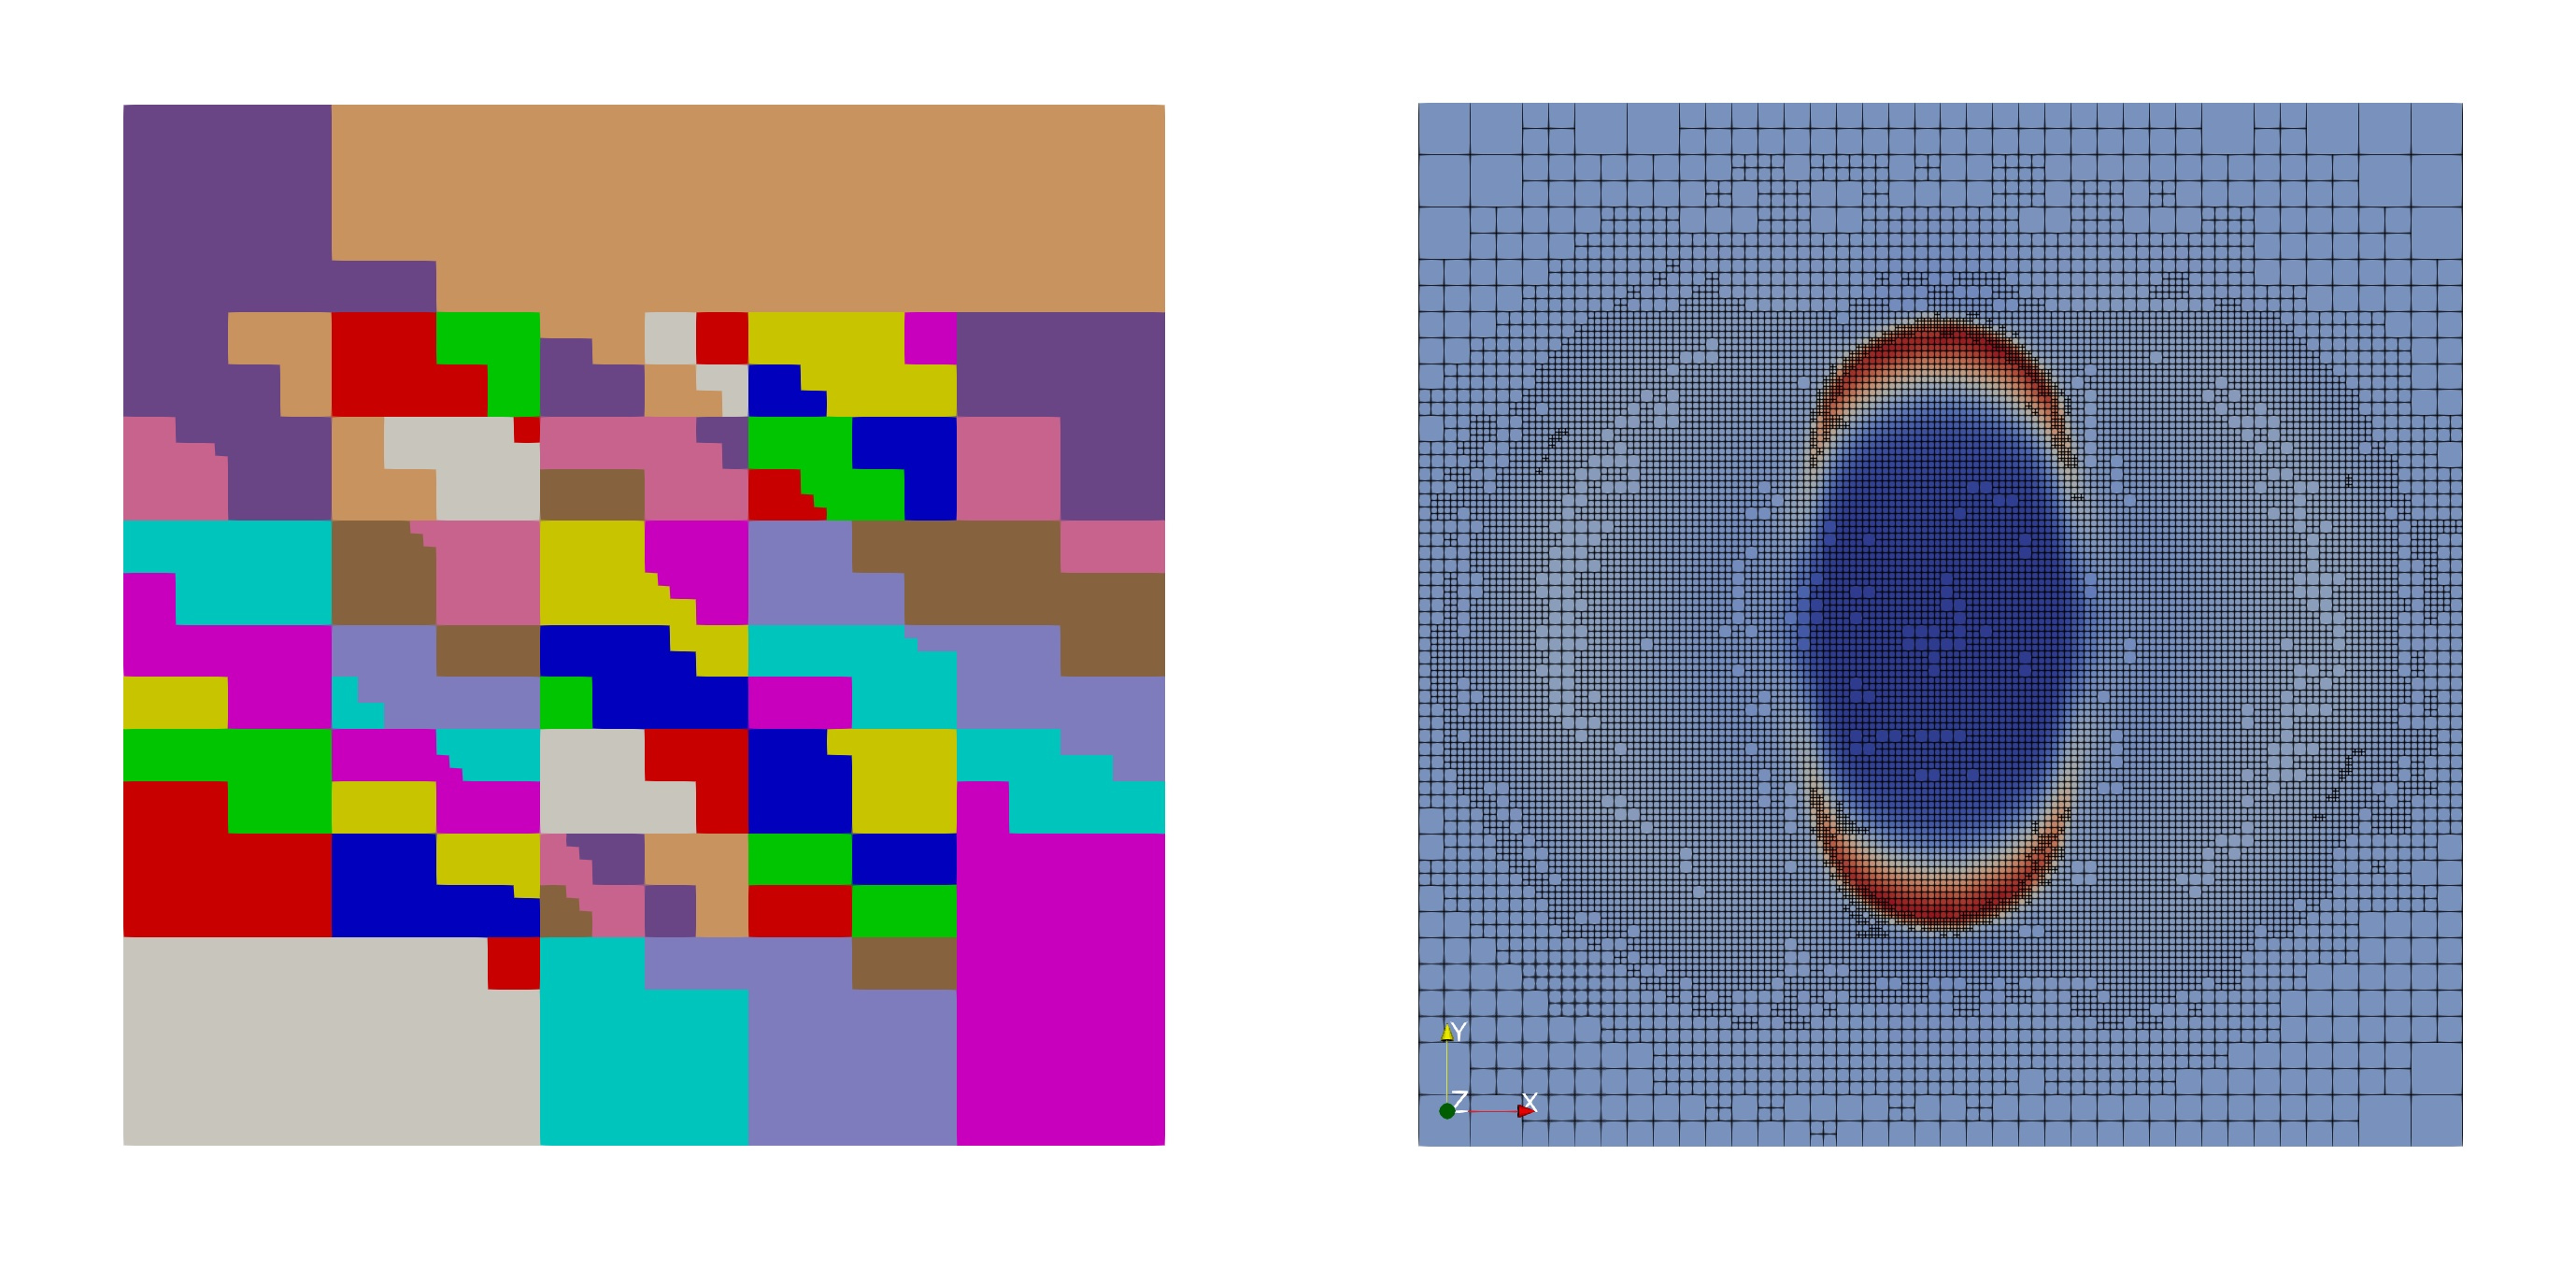
\includegraphics[width=0.87\textwidth]{img//mhd-blast/old/mya6.jpg}
	\caption{Obtained results, $t = 25\times 10^{-3}$, distribution of elements (right) to processors (left)}
	\label{figure:blastOldMyAdapt6}
	\end{center}
\end{figure}
\vspace{-8mm}

\subsubsection{MHD Blast - extended version}
\label{sec:blastNew}
An extended version of the benchmark has been used in \cite{blastNew1}, \cite{athenaBlast}, and a similar problem was used also in \cite{blastNew2} - the description of the benchmark is also available at:\url{http://www.astro.princeton.edu/~jstone/Athena/tests/blast/blast.html}.
In this version, the domain dimensions are set as a rectangle: $\Omega = [-0.5, 0.5] \times [-0.75, 0.75]$.
The initial conditions are a little different than in the case of \Cref{mhdBlastOld}, and read:
\begin{align}
\label{mhdBlastNew}
\gamma & =  5 / 3\\ \nonumber
p_0\lo\bfx, t\ro & =  10\ \ \text{for}\ \left|\bfx\right| < 0.1\\ \nonumber
p_0\lo\bfx, t\ro & =  0.1\ \ \text{for}\ \left|\bfx\right| \geq 0.1\\ \nonumber
\rho\lo\bfx, t = 0\ro & =  1,\\ \nonumber
p\lo\bfx, t = 0\ro & =  p_0\lo\bfx, t\ro,\\ \nonumber
\bfu_1\lo\bfx, t = 0\ro & =  0,\\ \nonumber
\bfu_2\lo\bfx, t = 0\ro & =  0,\\ \nonumber
\bfu_3\lo\bfx, t = 0\ro & =  0,\\ \nonumber
\bfB_1\lo\bfx, t = 0\ro & =  \frac{1}{\sqrt{2}},\\ \nonumber
\bfB_2\lo\bfx, t = 0\ro & =  \frac{1}{\sqrt{2}},\\ \nonumber
\bfB_3\lo\bfx, t = 0\ro & =  0,
\end{align}
with periodic boundary conditions on the top-bottom, and left-right parts of the boundary. That is, with respect to \Cref{periodicMapping}, the two pairs $\Gamma_1, \Gamma_2, \Gamma_1^{'}, \Gamma_2^{'}$ are specified as follows:
\begin{align}
\Gamma_1 & = \left\{-0.5\right\} \times [-0.75, 0.75],\\
\Gamma_2 & = \left\{0.5\right\} \times [-0.75, 0.75],
\end{align}
and
\begin{align}
\Gamma_1^{'} & = [-0.5, 0.5] \times \left\{-0.75\right\},\\
\Gamma_2^{'} & = [-0.5, 0.5] \times \left\{0.75\right\}.
\end{align}

\subsubsection{Calculation specification}
A mesh $T_h$ formed by rectangular hexahedra was used.
The value of the time step $\tau$ used was set according to the CFL condition (\Cref{section:CFL}).
Illustration of the obtained results follows below - these results were obtained using one node of the department's computational cluster with these parameters:
\begin{itemize}
    \item CPU: Intel(R) Xeon(R) CPU E5-2680 v3 @ 2.50GHz
    \item \# of Cores: 48 per node (nodes 1, 2), 16 per node (nodes 3, 4)
    \item Vectorization support: AVX2
    \item Parallelization implemented: Intel TBB
    \item Distributed calculation implemented: OpenMPI
    \item RAM: 512 GB
    \item OS: Ubuntu 15.10
\end{itemize}

\subsubsection{Results}
The results show distribution of plasma - $\rho$ in the domain.

TODO - moje vysledky Blastu\\
TODO - moje vysledky Blastu s adaptivitou\\

\subsection{Orszag-Tang vortex}
This problem was first described in \cite{vortex} and has been extensively used as a benchmark for 2- and 3- dimensional MHD code (\cite{blast0}, \cite{blast1}, \cite{honzaFem}, \cite{otnew}, and many others). It is a simple model of the evolution of MHD turbulence including interactions between the several shock waves that appear. The Orszag-Tang system is defined by the initial conditions:
\begin{align}
\rho_0 & =  \frac{25}{36 \pi}\\ \nonumber
p_0 & =  \frac{5}{12 \pi}\\  \nonumber
B_0 & =  \sqrt{\frac{1}{4 \pi}}\\ \nonumber
\gamma & =  5 / 3\\ \nonumber
\rho\lo\bfx, t = 0\ro & =  \rho_0,\\ \nonumber
p\lo\bfx, t = 0\ro & =  p_0,\\ \nonumber
\bfu_1\lo\bfx, t = 0\ro & =  -\sin(2 \pi y),\\ \nonumber
\bfu_2\lo\bfx, t = 0\ro & =  \sin(2 \pi x),\\ \nonumber
\bfu_3\lo\bfx, t = 0\ro & =  0,\\ \nonumber
\bfB_1\lo\bfx, t = 0\ro & =  -B_0 \sin(2 \pi y),\\ \nonumber
\bfB_2\lo\bfx, t = 0\ro & =  B_0 \sin(4 \pi x),\\ \nonumber
\bfB_3\lo\bfx, t = 0\ro & =  0,\\ \nonumber
U\lo\bfx, t = 0\ro & =  \frac{p_0}{\gamma - 1} + U_m\lo\bfx, t\ro + U_k\lo\bfx, t\ro,
\end{align}
where the last term is an application of \Cref{magU}, \Cref{kinU}, \Cref{presU}. The domain $\Omega$ is set as $\Omega = [0, 1] \times [0, 1]$ and the problem is equipped with periodic boundary conditions on the top-bottom, and left-right parts of the boundary, similarly as in \Cref{sec:blastNew}. This configuration is strongly unstable, leading to a wide spectrum of propagating MHD modes and shock waves.
\paragraph{}
As before, in order to compare with reference papers, figures are presented from these papers - see \Cref{figure:otRef}. The images are taken from pages 30 (\cite{blast1}), and 20/282 (\cite{blast0}) respectively. All are taken at $t = 0.5$.

\begin{figure}[H]
\centering
\subfigure{\vspace{12mm}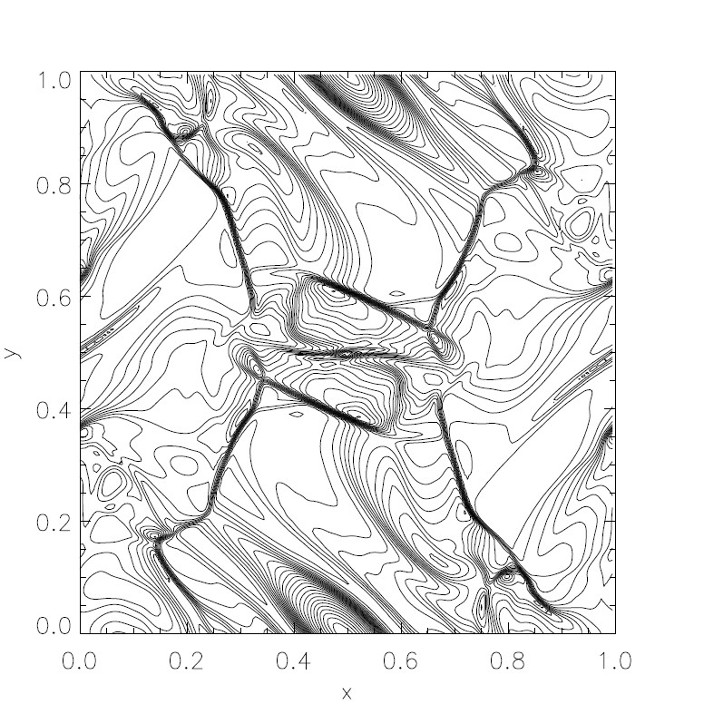
\includegraphics[width=0.4\textwidth]{img/ot/ref-londrillo-pressure.jpg}}
\subfigure{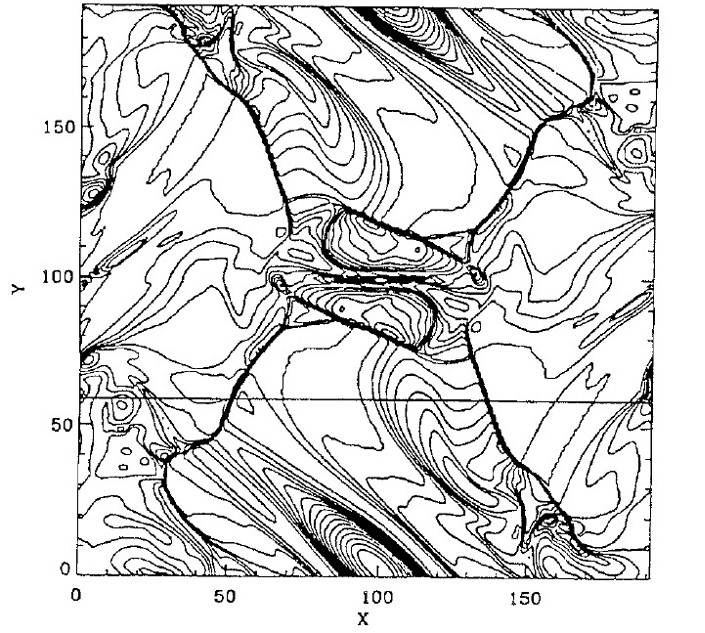
\includegraphics[width=0.4\textwidth]{img/ot/ref-zachary-pressure-contour.jpg}}\\
\subfigure{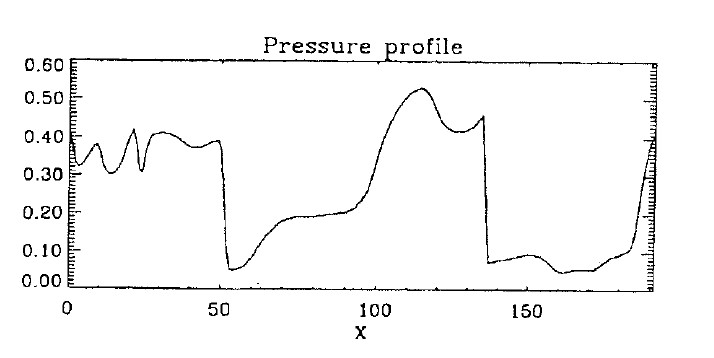
\includegraphics[width=0.75\textwidth]{img/ot/ref-zachary-pressure-profile.jpg}}
\caption{$p$ isolines from \cite{blast1} (top left), $p$ isolines from \cite{blast0} (top right), $p$ along $y = 0.3125$ from \cite{blast0} (bottom).}
\label{figure:otRef}
\end{figure}


TODO - vysledky z cite otnew\\
TODO - moje vysledky O-T\\
TODO - moje vysledky O-T s adaptivitou\\

\section{Flux tube eruption model}
This model is based on the original Titov-Demoulin model from \cite{td}, as used in \cite{miraClanek}.

The model parameters are as follows. Note that $k_B$ is the Boltzmann constant $k_B = 1.38064852 \times 10^{-23} \frac{\mathrm{J}}{\mathrm{K}}$, $m_p$ is the plasma mass, and $g$ gravitational acceleration.

\begin{align}
\beta & =  0.05\ \ \ \ ...\ \text{Plasma beta}\\
L_G & =  2\ k_B \frac{T_{ext}}{\lo m_p g \ro} = 1.2 \times 10^8 \left[\text{m}\right]\\
L_G & =  20 \ \ \ \ ...\ \text{Coronal height scale in dimension-less units}\\
\\
& !!! & \text{TODO - Proc je v kodu} L_G = 0.0 \ ?\
\\ \\
N_t & = -3\ \ \ \ ...\ \text{Torus winding number}\\
R & = 4\ \ \ \ ...\ \text{Torus major radius}\\
2L & =  4\ \ \ \ ...\ \text{Magnetic charge separation distance}\\
d & =  2\ \ \ \ ...\ \text{Geometrical factor}\\
q_{mag} & =  \left| \frac{\ln\lo 8 e^{-5/4} R\ro}{4} N_t \lo\frac{L}{R}\ro^2\left[1 + \lo\frac{R}{L}\ro^2\right]^{3/2}\right|\\
q_{mag} & \approx & \text{Normalised magnetic charge corresponding to global equilibrium}\\
q_{mag} & =  \frac{ \ln\lo 8R \ro - \frac{5}{4}}{4} \left| N_t \right| \frac{\lo 1 + \lo\frac{L}{R}\ro^2\ro \sqrt{1 + \lo\frac{L}{R}\ro^2}}{\frac{L}{R}}\\
\\
& !!! & \text{TODO - Neni toto spatne nakodene?}
\\\ \\
H & =  2\ \frac{N_t^2}{R^2}\ \ \ \ ...\ \text{"Helicity" factor inside tho loop}\\
\frac{ T_{ext} }{T_{in}} & =  10\ \ \ \ ...\ \text{Coronal/prominence temperature ratio}\\
\\
& !!! & \text{TODO - Proc je v kodu Tc2Tp = 1?}
\\\ \\
\end{align}